\documentclass[
	fontsize=12pt,           % Leitlinien sprechen von Schriftgröße 12.
	paper=A4,
	twoside=false,
	listof=totoc,            % Tabellen- und Abbildungsverzeichnis ins Inhaltsverzeichnis
	bibliography=totoc,      % Literaturverzeichnis ins Inhaltsverzeichnis aufnehmen
	titlepage,               % Titlepage-Umgebung anstatt \maketitle
	headsepline,             % horizontale Linie unter Kolumnentitel
	abstracton,              % Überschrift einschalten, Abstract muss in {abstract}-Umgebung stehen
]{scrreprt}                  % Verwendung von KOMA-Report
\usepackage[utf8]{inputenc}  % UTF8 Encoding einschalten
\usepackage[ngerman]{babel}  % Neue deutsche Rechtschreibung
\usepackage[T1]{fontenc}     % Ausgabe von westeuropäischen Zeichen (auch Umlaute)
\usepackage{mathpazo}         % Nicht-gerasterte Schriftarten (bei MikTeX erforderlich)
\usepackage{graphicx}        % Einbinden von Grafiken erlauben
\usepackage{wrapfig}         % Grafiken fließend im Text
\usepackage{setspace}        % Zeilenabstand \singlespacing, \onehalfspaceing, \doublespacing
\usepackage[
	%showframe,                % Ränder anzeigen lassen
	left=2.7cm, right=2.5cm,
	top=2.5cm,  bottom=2.5cm,
	includeheadfoot
]{geometry}                      % Seitenlayout einstellen
\usepackage{scrlayer-scrpage}    % Gestaltung von Fuß- und Kopfzeilen
\usepackage{acronym}             % Abkürzungen, Abkürzungsverzeichnis
\usepackage{titletoc}            % Anpassungen am Inhaltsverzeichnis
\contentsmargin{0.725cm}         % Abstand im Inhaltsverzeichnis zw. Punkt und Seitenzahl
\usepackage[                     % Klickbare Links (enth. auch "nameref", "url" Package)
  hidelinks,                     % Blende die "URL Boxen" aus.
  breaklinks=true                % Breche zu lange URLs am Zeilenende um
]{hyperref}
\urlstyle{same}                  % Aktuelle Schrift auch für URLs
% Anpassung von autoref für Gleichungen (ergänzt runde Klammern) und Algorithm.
% Anstatt "Listing" kann auch z.B. "Code-Ausschnitt" verwendet werden. Dies sollte
% jedoch synchron gehalten werden mit \lstlistingname (siehe weiter unten).
\addto\extrasngerman{%
	\def\equationautorefname~#1\null{Gleichung~(#1)\null}
	\def\lstnumberautorefname{Zeile}
	\def\lstlistingautorefname{Listing}
	\def\algorithmautorefname{Algorithmus}
	% Damit einheitlich "Abschnitt 1.2[.3]" verwendet wird und nicht "Unterabschnitt 1.2.3"
	% \def\subsectionautorefname{Abschnitt}
}

% ---- Abstand verkleinern von der Überschrift 
\renewcommand*{\chapterheadstartvskip}{\vspace*{.5\baselineskip}}

% Hierdurch werden Schusterjungen und Hurenkinder vermieden, d.h. einzelne Wörter
% auf der nächsten Seite oder in einer einzigen Zeile.
% LaTeX kann diese dennoch erzeugen, falls das Layout ansonsten nicht umsetzbar ist.
% Diese Werte sind aber gute Startwerte.
\widowpenalty10000
\clubpenalty10000

% ---- Für das Quellenverzeichnis
\usepackage[
	backend = biber,                % Verweis auf biber
	language = auto,
	style = numeric,                % Nummerierung der Quellen mit Zahlen
	sorting = none,                 % none = Sortierung nach der Erscheinung im Dokument
	sortcites = true,               % Sortiert die Quellen innerhalb eines cite-Befehls
	block = space,                  % Extra Leerzeichen zwischen Blocks
	hyperref = true,                % Links sind klickbar auch in der Quelle
	%backref = true,                % Referenz, auf den Text an die zitierte Stelle
	bibencoding = auto,
	giveninits = true,              % Vornamen werden abgekürzt
	doi=false,                      % DOI nicht anzeigen
	isbn=false,                     % ISBN nicht anzeigen
    alldates=short                  % Datum immer als DD.MM.YYYY anzeigen
]{biblatex}
\addbibresource{content/literatur.bib}
\setcounter{biburlnumpenalty}{3000}     % Umbruchgrenze für Zahlen
\setcounter{biburlucpenalty}{6000}      % Umbruchgrenze für Großbuchstaben
\setcounter{biburllcpenalty}{9000}      % Umbruchgrenze für Kleinbuchstaben
\DeclareNameAlias{default}{last-first}  % Nachname vor dem Vornamen
\AtBeginBibliography{\renewcommand{\multinamedelim}{\addslash\space
}\renewcommand{\finalnamedelim}{\multinamedelim}}  % Schrägstrich zwischen den Autorennamen
\DefineBibliographyStrings{german}{
  urlseen = {Einsichtnahme:},                      % Ändern des Titels von "besucht am"
}
\usepackage[babel,german=quotes]{csquotes}         % Deutsche Anführungszeichen + Zitate


% ---- Für Mathevorlage
\usepackage{amsmath}    % Erweiterung vom Mathe-Satz
\usepackage{amssymb}    % Lädt amsfonts und weitere Symbole
\usepackage{MnSymbol}   % Für Symbole, die in amssymb nicht enthalten sind.


% ---- Für Quellcodevorlage
\usepackage{scrhack}                    % Hack zur Verw. von listings in KOMA-Script
\usepackage{listings}                   % Darstellung von Quellcode
\usepackage{xcolor}                     % Einfache Verwendung von Farben
% -- Eigene Farben für den Quellcode
\definecolor{JavaLila}{rgb}{0.4,0.1,0.4}
\definecolor{JavaGruen}{rgb}{0.3,0.5,0.4}
\definecolor{JavaBlau}{rgb}{0.0,0.0,1.0}
\definecolor{ABAPKeywordsBlue}{HTML}{6000ff}
\definecolor{ABAPCommentGrey}{HTML}{808080}
\definecolor{ABAPStringGreen}{HTML}{4da619}
\definecolor{PyKeywordsBlue}{HTML}{0000AC}
\definecolor{PyCommentGrey}{HTML}{808080}
\definecolor{PyStringGreen}{HTML}{008080}

% -- Default Listing-Styles

\lstset{
	% Das Paket "listings" kann kein UTF-8. Deswegen werden hier 
	% die häufigsten Zeichen definiert (ä,ö,ü,...)
	literate=%
		{á}{{\'a}}1 {é}{{\'e}}1 {í}{{\'i}}1 {ó}{{\'o}}1 {ú}{{\'u}}1
		{Á}{{\'A}}1 {É}{{\'E}}1 {Í}{{\'I}}1 {Ó}{{\'O}}1 {Ú}{{\'U}}1
		{à}{{\`a}}1 {è}{{\`e}}1 {ì}{{\`i}}1 {ò}{{\`o}}1 {ù}{{\`u}}1
		{À}{{\`A}}1 {È}{{\'E}}1 {Ì}{{\`I}}1 {Ò}{{\`O}}1 {Ù}{{\`U}}1
		{ä}{{\"a}}1 {ë}{{\"e}}1 {ï}{{\"i}}1 {ö}{{\"o}}1 {ü}{{\"u}}1
		{Ä}{{\"A}}1 {Ë}{{\"E}}1 {Ï}{{\"I}}1 {Ö}{{\"O}}1 {Ü}{{\"U}}1
		{â}{{\^a}}1 {ê}{{\^e}}1 {î}{{\^i}}1 {ô}{{\^o}}1 {û}{{\^u}}1
		{Â}{{\^A}}1 {Ê}{{\^E}}1 {Î}{{\^I}}1 {Ô}{{\^O}}1 {Û}{{\^U}}1
		{œ}{{\oe}}1 {Œ}{{\OE}}1 {æ}{{\ae}}1 {Æ}{{\AE}}1 {ß}{{\ss}}1
		{ű}{{\H{u}}}1 {Ű}{{\H{U}}}1 {ő}{{\H{o}}}1 {Ő}{{\H{O}}}1
		{ç}{{\c c}}1 {Ç}{{\c C}}1 {ø}{{\o}}1 {å}{{\r a}}1 {Å}{{\r A}}1
		{€}{{\euro}}1 {£}{{\pounds}}1 {«}{{\guillemotleft}}1
		{»}{{\guillemotright}}1 {ñ}{{\~n}}1 {Ñ}{{\~N}}1 {¿}{{?`}}1,
	breaklines=true,        % Breche lange Zeilen um 
	breakatwhitespace=true, % Wenn möglich, bei Leerzeichen umbrechen
	% Symbol für Zeilenumbruch einfügen
	prebreak=\raisebox{0ex}[0ex][0ex]{\ensuremath{\rhookswarrow}},
	postbreak=\raisebox{0ex}[0ex][0ex]{\ensuremath{\rcurvearrowse\space}},
	tabsize=4,                                 % Setze die Breite eines Tabs
	basicstyle=\ttfamily\small,                % Grundsätzlicher Schriftstyle
	columns=fixed,                             % Besseres Schriftbild
	numbers=left,                              % Nummerierung der Zeilen
	%frame=single,                             % Umrandung des Codes
	showstringspaces=false,                    % Keine Leerzeichen hervorheben
	keywordstyle=\color{blue},
	ndkeywordstyle=\bfseries\color{darkgray},
	identifierstyle=\color{black},
	commentstyle=\itshape\color{JavaGruen},   % Kommentare in eigener Farbe
	stringstyle=\color{JavaBlau},             % Strings in eigener Farbe,
	captionpos=b,                             % Bild*unter*schrift
	xleftmargin=5.0ex
}

% ---- Eigener JAVA-Style für den Quellcode
\renewcommand{\ttdefault}{pcr}               % Schriftart, welche auch fett beinhaltet
\lstdefinestyle{EigenerJavaStyle}{
	language=Java,                             % Syntax Highlighting für Java
	%frame=single,                             % Umrandung des Codes
	keywordstyle=\bfseries\color{JavaLila},    % Keywords in eigener Farbe und fett
	commentstyle=\itshape\color{JavaGruen},    % Kommentare in eigener Farbe und italic
	stringstyle=\color{JavaBlau}               % Strings in eigener Farbe
}

% ---- Eigener ABAP-Style für den Quellcode
\renewcommand{\ttdefault}{pcr}
\lstdefinestyle{EigenerABAPStyle}{
	language=[R/3 6.10]ABAP,
	morestring=[b]\|,                          % Für Pipe-Strings
	morestring=[b]\`,                          % für Backtick-Strings
	keywordstyle=\bfseries\color{ABAPKeywordsBlue},
	commentstyle=\itshape\color{ABAPCommentGrey},
	stringstyle=\color{ABAPStringGreen},
	tabsize=2
}

% ---- Eigener Python-Style für den Quellcode
\renewcommand{\ttdefault}{pcr}
\lstdefinestyle{EigenerPythonStyle}{
	language=Python,
	columns=flexible,
	keywordstyle=\bfseries\color{PyKeywordsBlue},
	commentstyle=\itshape\color{PyCommentGrey},
	stringstyle=\color{PyStringGreen}
}  % Weitere Details sind ausgelagert

\usepackage{algorithm}                  % Für Algorithmen-Umgebung (ähnlich wie lstlistings Umgebung)
\usepackage{algpseudocode}              % Für Pseudocode. Füge "[noend]" hinzu, wenn du kein "endif",
                                        % etc. haben willst.

\makeatletter                           % Sorgt dafür, dass man @ in Namen verwenden kann.
                                        % Ansonsten gibt es in der nächsten Zeile einen Compilefehler.
\renewcommand{\ALG@name}{Algorithmus}   % Umbenennen von "Algorithm" im Header der Listings.
\makeatother                            % Zeichen wieder zurücksetzen
\renewcommand{\lstlistingname}{Listing} % Erlaubt das Umbenennen von "Listing" in anderen Titel.

% ---- Tabellen
\usepackage{booktabs}  % Für schönere Tabellen. Enthält neue Befehle wie \midrule
\usepackage{multirow}  % Mehrzeilige Tabellen
\usepackage{siunitx}   % Für SI Einheiten und das Ausrichten Nachkommastellen
\sisetup{loctolang=DE:ngerman, decimalsymbol=comma} % Damit ein Komma und kein Punkt verwendet wird.

% ---- Für Definitionsboxen in der Einleitung
\usepackage{amsthm}                     % Liefert die Grundlagen für Theoreme
\usepackage[framemethod=tikz]{mdframed} % Boxen für die Umrandung
% ---- Definition für Highlight Boxen

% ---- Grundsätzliche Definition zum Style
\newtheoremstyle{defi}
  {\topsep}         % Abstand oben
  {\topsep}         % Abstand unten
  {\normalfont}     % Schrift des Bodys
  {0pt}             % Einschub der ersten Zeile
  {\bfseries}       % Darstellung von der Schrift in der Überschrift
  {:}               % Trennzeichen zwischen Überschrift und Body
  {.5em}            % Abstand nach dem Trennzeichen zum Body Text
  {\thmname{#3}}    % Name in eckigen Klammern
\theoremstyle{defi}

% ------ Definition zum Strich vor eines Texts
\newmdtheoremenv[
  hidealllines = true,       % Rahmen komplett ausblenden
  leftline = true,           % Linie links einschalten
  innertopmargin = 0pt,      % Abstand oben
  innerbottommargin = 4pt,   % Abstand unten
  innerrightmargin = 0pt,    % Abstand rechts
  linewidth = 3pt,           % Linienbreite
  linecolor = gray!40,       % Linienfarbe
]{defStrich}{Definition}     % Name der des formats "defStrich"

% ------ Definition zum Eck-Kasten um einen Text
\newmdtheoremenv[
  hidealllines = true,
  innertopmargin = 6pt,
  linecolor = gray!40,
  singleextra={              % Eck-Markierungen für die Definition
    \draw[line width=3pt,gray!50,line cap=rect] (O|-P) -- +(1cm,0pt);
    \draw[line width=3pt,gray!50,line cap=rect] (O|-P) -- +(0pt,-1cm);
    \draw[line width=3pt,gray!50,line cap=rect] (O-|P) -- +(-1cm,0pt);
    \draw[line width=3pt,gray!50,line cap=rect] (O-|P) -- +(0pt,1cm);
  }
]{defEckKasten}{Definition}  % Name der des formats "defEckKasten"  % Weitere Details sind ausgelagert

% ---- Für Todo Notes
\usepackage{todonotes}


\usepackage{ifthen}
\newboolean{e-Abgabe}
\setboolean{e-Abgabe}{false}    % false=gedruckte Fassung

% ---- Persönlichen Daten:
\newcommand{\titel}{Digitalisierung von Reisen durch Entwicklung einer intelligenten Reiseführer App}
\newcommand{\titelheader}{Entwicklung einer intelligenten Reiseführer App}
\newcommand{\arbeit}{Studienarbeit}
\newcommand{\studiengang}{Angewandte Informatik}
\newcommand{\studienjahr}{2017}
\newcommand{\autor}{Joshua Schulz und Raphael Müßeler}
\newcommand{\autorReverse}{Schulz, Joshua; Müßeler, Raphael}
\newcommand{\verfassungsort}{Karlsruhe}
\newcommand{\matrikelnr}{4508858, 6801150}
\newcommand{\kurs}{TINF17B2}
\newcommand{\bearbeitungsmonat}{2020}
\newcommand{\abgabe}{18. Mai 2020}
\newcommand{\bearbeitungszeitraum}{01.10.2019 - 18.05.2020}
\newcommand{\firmaName}{SAP SE}
\newcommand{\firmaStrasse}{Dietmar-Hopp-Allee 16}
\newcommand{\firmaPlz}{69190 Walldorf, Deutschland}
\newcommand{\betreuerDhbw}{Thorsten Schlachter}

% ---- Metainformation für das PDF Dokument
\hypersetup{
	pdftitle    = {\titel},
	pdfsubject  = {\arbeit},
	pdfauthor   = {\autor},
	%pdfkeywords = {Keywords angeben},
	pdfcreator  = {LaTeX},
	%pdfproducer = {in der Regel pdfTeX}
}

% ---- Definition der Kopf- und Fußzeilen
\clearscrheadfoot                               % Löschen von LaTeX Standard
\automark[section]{chapter}                     % Füllen von section und chapter
\renewcommand*{\chaptermarkformat}{}            % Entfernt die Kapitelnummer
\renewcommand*{\sectionmarkformat}{}            % Entfernt die Sectionnummer
% Angaben [für "plain"]{für "scrheadings"}
\ihead[]{\titelheader}                          % Kopfzeile links
\chead[]{}                                      % Kopfzeile mitte
\ohead[]{\rightmark}                            % Kopfzeile rechts
\ifoot[]{}                                      % Fußzeile links
\cfoot*{\sffamily\pagemark}                     % Fußzeile mitte
\ofoot[]{}                                      % Fußzeile rechts
\KOMAoptions{
   headsepline = 0.2pt,                         % Liniendicke Kopfzeile
   footsepline = false                          % Liniendicke Fußzeile
}

% ---- Hilfreiches
\newcommand{\zB}{z.\,B. }   % "z.B." mit kleinem Leeraum dazwischen (ohne wäre nicht korrekt)
\newcommand{\dash}{d.\,h. }

\newcommand{\code}[1]{\texttt{#1}} % Ist einfacher zu schreiben als ständig \texttt und erlaubt
                                   % Änderungen im Nachhinein, wenn man z.B. Inline-Code anders stylen möchte.

% ---- Beginn des Dokuments
\begin{document}
\setlength{\parindent}{0pt}              % Keine Paragraphen Einrückung.
                                         % Dafür haben wir den Abstand zwischen den Paragraphen.
\setcounter{secnumdepth}{2}              % Nummerierungstiefe fürs Inhaltsverzeichnis
\setcounter{tocdepth}{1}                 % Tiefe des Inhaltsverzeichnisses. Ggf. so anpassen,
                                         % dass das Verzeichnis auf eine Seite passt.
\sffamily                                % Serifenlose Schrift verwenden.

% ---- Vorspann
% ------ Titelseite
\singlespacing
\thispagestyle{empty}
\begin{titlepage}
\enlargethispage{4cm}

\begin{figure}           % Logo vom Ausbildungsbetrieb und der DHBW
	% \vspace*{-5mm} % Sollte dein Titel zu lang werden, kannst du mit diesem "Hack" 
	%                  den Inhalt der Seite nach oben schieben.
	\begin{minipage}{0.49\textwidth}
		\flushleft
		
\includegraphics[height=2.5cm]{../logo/travlyn_logo.png} 
	\end{minipage}
	\hfill
	\begin{minipage}{0.49\textwidth}
		\flushright
		
\includegraphics[height=2.5cm]{images/Logos/Logo_DHBW.pdf} 
	\end{minipage}
\end{figure} 
\vspace*{0.1cm}

\begin{center}
	\huge{\textbf{\titel}}\\[1.5cm]
	\Large{\textbf{\arbeit}}\\[0.5cm]
	\normalsize{im Rahmen der Prüfung zum\\[1ex] \textbf{Bachelor of Science (B.Sc.)}}\\[0.5cm]
	\Large{des Studienganges \studiengang}\\[1ex]
	\normalsize{an der Dualen Hochschule Baden-Württemberg Karlsruhe}\\[1cm]
	\normalsize{von}\\[1ex] \Large{\textbf{\autor}} \\[1cm]
	\normalsize{\bearbeitungsmonat}\\[1ex] \Large{\textbf{-Sperrvermerk-}}\\[0.5cm]
\end{center}

\begin{center}
	\vfill
	\begin{tabular}{ll}
		Abgabedatum:                     & \abgabe \\[0.2cm]
		Bearbeitungszeitraum:            & \bearbeitungszeitraum \\[0.2cm]
		Matrikelnummer, Kurs:            & \matrikelnr , \kurs \\[0.2cm]
		Ausbildungsfirma:                & \firmaName \\
		                                 & \firmaStrasse \\
		                                 & \firmaPlz \\[0.2cm]
		Gutachter der Dualen Hochschule: & \betreuerDhbw \\[2cm]
	\end{tabular} 
\end{center}
\end{titlepage}
  % Titelseite
\newcounter{savepage}
\pagenumbering{Roman}                    % Römische Seitenzahlen
\onehalfspacing

% ------ Erklärung, Sperrvermerk, Abstact
\chapter*{Eidesstattliche Erklärung}
Ich versichere hiermit, dass ich meine \arbeit{} mit dem Thema:
\begin{quote}
	\textit{\titel}
\end{quote} 
gemäß § 5 der \enquote{Studien- und Prüfungsordnung DHBW Technik} vom 29. September 2017 selbstständig verfasst und keine anderen als die angegebenen Quellen und Hilfsmittel benutzt habe. Die Arbeit wurde bisher keiner anderen Prüfungsbehörde vorgelegt und auch nicht veröffentlicht.

\vspace{0.25cm}

Ich versichere zudem, dass die eingereichte elektronische Fassung mit der gedruckten Fassung übereinstimmt.

\vspace{1cm}

\verfassungsort, den \today \\[0.5cm]
\ifthenelse{\boolean{e-Abgabe}}
	{\underline{Gez. \autor}}
	{\makebox[6cm]{\hrulefill}}\\ 
\autorReverse

%\renewcommand{\abstractname}{Abstract} % Veränderter Name für das Abstract
\begin{abstract}
\begin{addmargin}[1.5cm]{1.5cm}        % Erhöhte Ränder, für Abstract Look
\thispagestyle{plain}                  % Seitenzahl auf der Abstract Seite

\begin{center}
\small\textit{- English -}             % Angabe der Sprache für das Abstract
\end{center}

\vspace{0.25cm}

This is the starting point of the Abstract. For the final bachelor thesis, there must be an abstract included in your document. So, start now writing it in German and English. The abstract is a short summary with around 200 to 250 words.

\vspace{0.25cm}

Try to include in this abstract the main question of your work, the methods you used or the main results of your work.


\end{addmargin}
\end{abstract}
%\renewcommand{\abstractname}{Abstract} % Veränderter Name für das Abstract
\begin{abstract}
\begin{addmargin}[1.5cm]{1.5cm}        % Erhöhte Ränder, für Abstract Look
\thispagestyle{plain}                  % Seitenzahl auf der Abstract Seite

\begin{center}
\small\textit{- Deutsch -}             % Angabe der Sprache für das Abstract
\end{center}

\vspace{0.25cm}

Dies ist der Beginn des Abstracts. Für die finale Bachelorarbeit musst du ein Abstract in deinem Dokument mit einbauen. So, schreibe es am besten jetzt in Deutsch und Englisch. Das Abstract ist eine kurze Zusammenfassung mit ca. 200 bis 250 Wörtern.

\vspace{0.25cm}

Versuche in das Abstract folgende Punkte aufzunehmen: Fragestellung der Arbeit, methodische Vorgehensweise oder die Hauptergebnisse deiner Arbeit.


\end{addmargin}
\end{abstract}

% ------ Inhaltsverzeichnis
\singlespacing
\tableofcontents

% ------ Verzeichnisse
\renewcommand*{\chapterpagestyle}{plain}
\pagestyle{plain}
%\include{content/03_listings/formelgroessen}
\chapter*{Abkürzungsverzeichnis}
\addcontentsline{toc}{chapter}{Abkürzungsverzeichnis} % Hinzufügen zum Inhaltsverzeichnis 

\begin{acronym}[WYSISWG] % längstes Kürzel wird verw. für den Abstand zw. Kürzel u. Text

	% Alphabetisch selbst sortieren - nicht verwendete Kürzel rausnehmen!

	\acro{AOP}{Aspect-oriented Programming}
	\acro{API}{Application Programming Interface}
	\acro{HTTP}{Hypertext Transfer Protocol}
	\acro{IO}{Input/Output}
	\acro{IoC}{Inversion of Control}
	\acro{JPA}{Java Persistence API}
	\acro{JTA}{Java Transaction API}
	\acro{JVM}{Java Virtual Machine}
	\acro{OAI}{OpenAPI}
	\acro{ORM}{Object-relational Mapping}
	\acro{POI}{Point of interest}
	\acro{REST}{Representational State Transfer}
	\acro{RPC}{Remote Procedure Call}
	\acro{SDK}{Software Development Kit}
	\acro{SOAP}{Simple Objec Access Protocol}
	\acro{SQL}{Structured Query Language}
	\acro{UI}{User Interface}
	\acro{URI}{Uniform Resource Identifier}
	\acro{WWW}{World Wide Web}
	\acro{XML}{Extensible Markup Language}
	\acro{YAML}{YAML Ain’t Markup Language}

\end{acronym}
\listoffigures                          % Erzeugen des Abbildungsverzeichnisses 
\listoftables                           % Erzeugen des Tabellenverzeichnisses
\renewcommand{\lstlistlistingname}{Quellcodeverzeichnis}
\lstlistoflistings                      % Erzeugen des Listenverzeichnisses
\setcounter{savepage}{\value{page}}


% ---- Inhalt der Arbeit
\cleardoublepage
\pagenumbering{arabic}                  % Arabische Seitenzahlen für den Hauptteil
\setlength{\parskip}{0.5\baselineskip}  % Abstand zwischen Absätzen
\rmfamily
\renewcommand*{\chapterpagestyle}{scrheadings}
\pagestyle{scrheadings}
\onehalfspacing
\chapter{Einleitung}

	(Joshua)

	In der heutige Zeit unterliegt die Welt der Medien einer sehr rasanten und starken Veränderung. Es werden immer mehr neuartige und innovative Techniken entwickelt, wie Medien konsumiert werden können, z.B. Augmented und Virtual Reality. Durch diese Techniken wird versucht die Mediennutzung effektiver, intensiver und moderner zu machen. In vielen Bereichen haben diese Techniken bereits Einzug gehalten und sind für eine große Masse von Konsumenten verfügbar, z.B. Virtual Reality gaming mit Hilfsmitteln wie Oculus Rift \cite{OculusVR.3222020} und anderen Produkten.

	\vspace{0.25cm}

	Allerdings gibt es ebenfalls Bereiche bei denen die Digitalisierung und Nutzung neuer Techniken nicht komplett ausgenutzt werden und viele weitere Vorteile ungenutzt bleiben, wie z.B. beim Reisen \cite{Dredge.}: Viele Menschen nutzen Reiseführer, um sich einen Überblick über ihre Reisedestination zu verschaffen und einen grundlegenden Plan zu erstellen, allerdings findet man diese Reiseführer fast ausschließlich in gedruckter Buchform. Das bedeutet für die Buchform, dass immer schwere Printmedien mit in den Urlaub genommen werden müssen, dass Informationen in den Reiseführern nicht aktualisiert werden können, ohne eine neue Auflage herauszugeben und eine interaktive Gestaltung der Medien nicht möglich ist. Außerdem sind die Seiten in einem Buch begrenzt, d.h. es muss für jede Reise ein neuer Reiseführer erworben werden, der spezielle Informationen zum Reiseziel enthält. All dies sind Nachteile, die durch eine Digitalisierung der Inhalte ausgeglichen werden könnten: Das Smartphone ist heutzutage ein ständiger Begleiter, der ausgenutzt werden kann, um Echtzeitinformationen schnell und immer aktuell zur Verfügung zu stellen. Außerdem können interaktive Elemente wie Karten, Navigation, Audioguides uvm. direkt integriert werden. Es wäre möglich einen Anwendung zu schaffen, die in der Lage ist, für jede beliebige Stadt und Region auf der Welt Informationen bereit zu stellen, ohne dass neue Inhalte erworben werden müssen. Als Geschäftsmodel des Anbieters wäre es denkbar Geld durch den Einsatz von Werbung zu verdienen oder durch Bezahlung von Städten im Gegenzug für besondere Herausstellung innerhalb der Anwendung.  Damit könnte eine Reise entstehen, die unkomplizierter und trotzdem viel aktueller ist als bei Benutzung eines herkömmlichen Reiseführers.

	\vspace{0.25cm}

	Es könnten viele Services, die aktuell parallel zum Reiseführer genutzt werden (z.B. verschiedene Bewertungsportale und Karten) direkt integriert werden, um alle Informationen auf einen Blick zur Verfügung zu stellen. Ebenso könnte eine Personalisierung der verfügbaren Daten umgesetzt werden. Im Gegensatz zum herkömmlichen Reiseführer, welcher allgemeine und damit u.U. viele für den einzelnen irrelevant Informationen enthält, werden Vorschläge anhand der vom Nutzer gesetzten Vorlieben gemacht und somit nur nützliche Informationen zur Verfügung gestellt.

	\vspace{0.25cm}

	Insgesamt soll ein digitaler Reiseführer entstehen, der das Reiseerlebnis auf eine bessere, digitalere und einfachere Ebene hebt und noch mehr Spaß am Reisen erzeugen kann.

	\section{Motivation}

	Wir möchten mit dieser Arbeit einen Beitrag zu einer digitalisierten und technisch geprägten Gesellschaft leisten, indem wir eine Anwendung schaffen, die mit den Nachteilen von gedruckten Reiseführern aufräumt und eine neue innovative Art des Reisen schafft. Damit soll das Reiseerlebnis der Menschen verbessert werden und ihnen die Möglichkeit geben sich noch mehr auf das Erlebte zu konzentrieren, ohne Gedanken an eine komplizierte Planung, bei der viele Medien parallel genutzt werden, zu verschwenden.
	Außerdem ist diese Arbeit Teil unserer Prüfung zum Bachelor of Science und dient zur praktischen Anwendung der bisher im Studium erlernten Fähigkeiten und zum Ausprobieren neuer innovativer Techniken um unser Wissen zu erweitern.   

	\section{Gliederung der Arbeit}
	
	In dieser Arbeit soll die durchgeführte Entwicklung detailliert beschrieben und festgehalten werden. Dazu werden alle wichtigen Arbeitsschritte aufgeschlüsselt und die Ergebnisse entsprechend dargestellt. Die entwickelte App trägt den Namen \textit{Travlyn} und wird im Verlauf dieser Arbeit nur noch so bezeichnet. Dieser Name entstand bei Diskussionen der Teammitglieder und wurde für markenfähig befunden. 
	
	\vspace{0.25cm}
	
	An erster Stelle steht die Beschreibung der verwendeten Techniken, Prozessen und Begriffen. An dieser Stelle werden alle, für diese Arbeit, relevanten Eigenschaften genannt und Verweise auf weiterführende Literatur geliefert um ein gemeinsame Ausgangslage zu schaffen. Anschließend werden die Anforderungen an die zu entwickelnde App geschildert und Ziele gesetzt, die erreicht werden sollen. Danach wird auf ein sehr zentrales Thema dieser Entwicklung eingegangen: Die Datenquellen. Ein Reiseführer lebt von den präsentierten Daten und somit ist die Auswahl der Datenquellen anhand der Anforderungen von großer Bedeutung. Ein ähnliches Gewicht hat das erstellen eines Übergeordneten Konzepts für die Anwendung und dessen Spezialisierung auf kleinere Komponenten der Software. Das Ergebnis dieses Prozesses wird im Anschluss an die Datenquellen ausführlich dargestellt. Nach der Konzeption folgt die Durchführung und Implementation, von der nur einige zentrale und/oder kritische Punkte dargestellt werden. Abschließend soll das entstandene Ergebnis anhand bestimmter Verfahren evaluiert werden und gegen die zu Beginn definierten Ziele validiert werden. Nach dieser Evaluation mündet diese Arbeit in ein Fazit, welches einen Ausblick auf zukünftige Erweiterung und Verbesserungen gibt und zentrale Punkte, die das Team aus diesem Projekt mitgenommen hat, darstellt.  

\chapter{Voraussetzungen}

%	\section{Machine Learning}
	
	\section{RESTful APIs} % Raphael
	
		Representational State Transfer beschreibt ein architektonisches Modell, um Web Services zu erstellen. Sogenannte \ac{REST} Web Services bieten Interoperabilität zwischen Computersystemen im Internet -- geeignet für die Kommunikation von Maschine zu Maschine. So lässt sich REST auch als eine Abstraktion der Struktur und des Verhaltens des World Wide Webs beschreiben. 
		
		Neben REST gibt es weitere Alternativen, wie \ac{SOAP} oder \ac{RPC}; der Vorteil von REST besteht jedoch darin, dass durch das \ac{WWW} ein Großteil der Infrastruktur für die Kommunikation bereits vorhanden und implementiert ist. Während bei \\ac{RPC} in der \ac{URI} Methodeninformationen enthalten sind, gibt eine \ac{URI} in der \ac{REST} Architektur ausschließlich Ressourcen an und kodiert die Funktionalität mittels \ac{HTTP} Methoden. Dieser Ansatz entspricht dem Konzept einer \ac{URI}, da bei einer \ac{HTTP} Anfrage ebenso nur Ressourcen und keine Funktionalität gefragt ist.
		
		Eine REST API muss insgesamt sechs Eigenschaften besitzen:
		
		\begin{description}
			\item[Client-Server Architektur] 
				Bei \ac{REST} gilt im Allgemeinen, dass eine Client-Server Architektur vorliegen soll: Die Client konsumiert die vom Server bereitgestellten Dienste. 
			\item[Zustandslosigkeit] 
				Eine RESTful \ac{API} soll keine Zustände haben, sondern so konzipiert werden, dass benötigten Informationen in einer REST-Nachricht enthalten sind. Dies begünstigt außerdem die Skalierbarkeit eines solchen Dienstes, da es auf diese Weise einfacher ist, alle Anfragen auf mehrere Instanzen zu verteilen.
			\item[Caching] 
				Server sowie Client können Antworten zwischenspeichern. Es muss jedoch vorher explizit definiert werden, welche Antworten zwischengespeichert und welche nicht zwischengespeichert werden, um zu verhindern, dass alte oder ungeeignete Daten versendet werden.
			\item[Einheitliche Schnittstelle]
				Die \ac{REST} \ac{API} muss eine einheitliche Schnittstelle zur Verfügung stellen, welche den von \cite{RoyThomasFielding.2000} definierten Anforderungen entsprechen muss. Dies vereinfacht die Nutzung der \ac{API}.
			\item[Mehrschichtige Systeme]
				 Die Struktur einer RESTful \ac{API} soll mehrschichtig sein, sodass es ausreicht, dem Client lediglich eine Schnittstelle anzubieten. Die Architektur der API wird dadurch simplifiziert und die dahinterliegenden Schichten der Implementierung bleiben verborgen.
			\item[Code on Demand] 
				Fielding beschreibt diese Eigenschaft als optional: Der Server kann, durch das Übertragen von ausführbarem Code, die Funktionalität des Clients zeitweise erweitern oder anpassen. Vorstellbar wäre beispielsweise eine Übertragung von bereits kompilierten Komponenten oder Client-seitigen Skripten. 
				
		\end{description}

	\section{Frameworks}
	
		\subsection{OpenAPI} % Raphael
		
			Der OpenAPI Standard ist Open Source und dient der Beschreibung von RESTful APIs. Bis 2016 war OpenAPI Teil des Swagger Frameworks, wurde schließlich aber als separates Projekt unter Aufsicht der sog. \textit{OpenAPI Initiative}  ausgelagert. 
			
			Mit der deklarativen Ressourcenspezifikation von OpenAPI können Clients Dienste verstehen und konsumieren, ohne über Kenntnisse der eigentlichen Server-Implementierung bzw. Zugriff auf den Servercode zu verfügen. Dies erleichtert die Entwicklung Client-seitiger Applikationen, die RESTful APIs verwenden. Die OpenAPI-Spezifikation ist zudem sprachunabhängig und lässt sich in jeder Beschreibungssprache (\ac{YAML}, \ac{XML} etc.) definieren. 
	
		\subsection{Swagger} % Raphael
		
			Swagger ist ein Framework das sich des OpenAPI Standards bedient. Swagger bietet ein Tooling an, mit dessen Hilfe APIs spezifiziert und beschrieben werden können. Neben einem entsprechenden Editor, bietet Swagger die Möglichkeit, aus der OpenAPI Spezifikation Code zu generieren und zwar unter Verwendung unterschiedlicher Frameworks -- z.B. eine vollständige Spring Applikation -- wobei nur noch die eigentliche Implementierung der Businesslogik erforderlich ist.
			
			Des Weiteren stellt Swagger eine Web-basierte Benutzeroberfläche zur Verfügung, welche nicht nur die direkte Anbindung von Live APIs ermöglicht, sondern auch eine visuelle Dokumentation der \ac{API} darstellt. \cite{SmartBear.2020}
	
		\subsection{Spring} % Raphael
		
			Spring ist ein Open Source Framework, welches in Java geschrieben wurde. Es gilt als de facto Standard bei der Entwicklung von RESTful API, da es in der Open Source Welt viel Zuspruch und Verwendung gefunden hat. Zudem integriert Spring mit fast allen Java Umgebungen und ist somit nicht nur für Anwendungen im kleinen Maßstab, sondern eben so für Anwendungen in großen Unternehmen geeignet. \cite{Walls.20162017} 
			
			Bei der Entwicklung dieses Frameworks wurden die unter anderem in \cite{Johnson.2003} beschriebenen Design Prinzipien mithilfe der folgenden Module und deren entsprechender Funktionalität umgesetzt:
			
			\subsubsection{Dependency Injection} % Raphael
			
				Der von Martin Fowler 2004 definierte Begriff der \textit{Dependency Injection} ist eine Präzisierung oder Spezialisierung des Begriffs \textit{Inversion of Control}. \ac{IoC} bezeichnet ein Paradigma, welches den Kontrollfluss einer Applikation nicht mehr der Anwendung, sondern dem Framework -- in diesem Fall Spring -- überlässt. Ein Beispiel für \ac{IoC} sind Listener (Beobachter Muster). \\
				Dependency Injection beschreibt ein Entwurfsmuster, bei welchem festgelegte Abhängigkeiten nicht zur Kompilierzeit, sondern zur Laufzeit bereitgestellt werden. Dies lässt sich einem Beispiel erläutern: Besteht bei der Initialisierung eines Objektes eine Abhängigkeit zu einem anderen Objekt, so wird diese Abhängigkeit an einem zentralen Ort hinterlegt. Wenn nun die Initialisierung dieses Objektes erfolgt, beauftragt es den sog. Injector (dt. Injezierer), die Abhängigkeit aufzulösen. \cite{MartinFowler.23.01.2020}
				
				In Spring bietet der \ac{IoC} Container mittels Reflexion ein konsistentes Werkzeug zur Konfiguration sowie Verwaltung von Java Objekten. Diese durch den Container erstellten Objekten heißen \textit{Beans}. Die Konfiguration des Containers erfolgt entweder über eine \ac{XML} Datei oder über Java Annotationen. \cite{Walls.20162017} 
				
			\subsubsection{Aspektorientierte Programmierung}
			
				\ac{AOP} beschreibt ein Paradigma und ermöglicht die klassenübergreifende Verwendung generischer Funktionalität. Die führt zu einer starken Modularisierung und es gibt eine klare Trennung zwischen der Anwendungslogik und der Businesslogik (Cross-cutting Concern). \cite{Wunderlich.2005} \\
				Das Schreiben von Logs stellt ein Beispiel für ein Cross-cutting Concern dar, da eine Logging-Strategie alle protokollierten Klassen und Methoden erfasst und somit durchaus mit der Anwendungs- sowie der Businesslogik in Berührung kommt. 
			
			\subsubsection{Transaktionsmanagement} % Raphael
			\label{frameworks.spring.transaktionsmanagement}
			
				Ein weiteres Beispiel für \ac{AOP} ist sog. Transaktionsmanagement. Eine Transaktion bezeichnet in der Informatik eine logische Einheit, mit dessen Hilfe Aktionen auf einer Persistenz ausgeführt werden können. Dabei ist sichergestellt, dass sobald die Transaktion fehlerfrei und vollständig abgeschlossen ist, der Datenbestand weiterhin konsistent ist. Im Umkehrschluss bedeutet das, dass eine Transaktion entweder vollständig oder gar nicht ausgeführt wird. \cite{Ozsu.2011}
			
				Das von Spring bereitgestellte Transaktionsmanagement stellt eine Abstraktion auf die Java Plattform dar und ist in der Lage mit globalen und verschachtelten Transaktionen sowie sog. Savepoints -- ein Punkt innerhalb einer Transaktion, zu welchem im Fehlerfall zurück gesprungen werden kann -- zu arbeiten. Außerdem lasst sich diese Abstraktion in fast allen Java Umgebungen einsetzen. Die von Java bereitgestellte Java Transaction API (\ac{JTA}) hingegen unterstützt nur globale und verschachtelte Transaktionen und erfordert zudem immer einen Applikationsserver. 
			
			\subsubsection{Model View Controller} % Raphael
			
				Das \ac{MVC} (Model View Controller) Pattern ist ein weit verbreiteter Mechanismus zur Entwicklung von Benutzeroberflächen. \ac{MVC} stellt ein Design Pattern dar, dass Kapselung sowie eine Struktur für eine Architektur von Benutzeroberflächen bietet und bei welcher jeder Bereich eine definierte Aufgabe hat. Eine Verletzung der Zuständigkeitsbereiche ist zu vermeiden. \cite{Gamma.1995}
			
				Das Pattern besagt, dass die Architektur von Benutzerschnittstellen in folgende Bereiche aufgeteilt ist: Das \textit{Model} ist für den Zugriff auf die Datenbank und die Beschaffung von Daten zuständig. Häufig ist das Model auch für die Aufbereitung der Daten zuständig. Somit liegt die meist aufwändige Logik nicht beim Client, sondern bei den Servern, welche zumeist auch mit besserer Hardware ausgestattet sind. \\
				Ein \textit{Controller} definiert die Art und Weise, wie die Benutzerschnittstelle auf die Eingaben des Benutzer reagiert. Des Weiteren ist ein Controller für das Aktualisieren der Daten im Datenmodell, aber auch auf dem View zuständig. \\
				Der \textit{View} bestimmt ausschließlich, wie die Benutzeroberfläche aussehen soll. Er enthält -- in den meisten Implementierungen -- keine Logik, sondern ist lediglich eine Definition und Anordnung der Benutzeroberflächenelemente.
				
				Spring definiert für alle Verantwortlichkeiten eigene Strategie-Interfaces, wie beispielsweise das Controller Interface, welches alle eingehenden \ac{HTTP} Requests definiert und darüber hinaus auch behandelt. 

		
		\subsection{Hibernate} % Raphael
		
			Hibernate ist ein Persistenz- und Object-relational Mapping (\ac{ORM}) Framework, das ebenfalls unter einer Open Source Lizenz veröffentlicht und in Java geschrieben ist. Hibernate bietet eine Abstraktionsstufe gegenüber relationalen Datenbankimplementationen. Mithilfe der Sprache \textit{Hibernate Query Language} und dem entsprechend konfigurierten Dialekt (z.B. MySQL Dialekt, MariaDB Dialekt etc.) werden die entsprechenden Statements erzeugt und schließlich ausgeführt. Dies ermöglicht den einfach und schnellen Umstieg von einer Datenbankimplementation auf die andere, ohne Anpassung der sich im Code befindlichen Queries. 
			
			\subsubsection{Object-relational Mapping} % Raphael
		
				Eine häufig eingesetzt Technik der Persistierung sind relationale und meist auch \ac{SQL} basierte Datenbanken wie beispielsweise MySQL oder MariaDB. Wenn jedoch die Anwendung, welche die Businesslogik enthält, der Objektorientierung folgt, kommt es zu einem Widerspruch -- dem sog. Object-relational impendance mismatch --, welcher in den unterschiedlichen Paradigmen begründet liegt. So beschreibt die Objektrelationale Abbildung eine Technik, bei welcher sich Objekte einer objektorientierten Sprache in einer relationalen Datenbank persistieren lassen. 
					
				Java bietet mit der sog. Java Persistence API (\ac{JPA}) eine Abstraktion genau zu diesem Zweck, dessen sich Hibernate auch bedient. Mittels Annotationen lassen sich Objekte mit Attributen und Methoden -- zumeist Plain Old Java Objects (\ac{POJO}s) -- auf Entitäten abbilden. Diese Annotation definieren, welche Tabelle auf welches Objekt und welche Spalte auf welches Attribute abgebildet wird. Es lassen sich außerdem die Relationen der Entitäten auf die Assoziationen der Objekte abbilden. Hibernate bzw.\ac{JPA} unterstützt 1:1, 1:N sowie N:N Relationen. Somit wird ein vollständiges Abbild der Persistenz in der Anwendung geschaffen.
				
				Die einzige Vorgabe bei der Definition der Objekte ist, dass ein parameterloser Konstruktor existieren muss. Hibernate greift auf die Attribute der Klasse mittels Reflexion zu. 
				
			\subsubsection{Transaktionsmanagement} % Raphael
			
				In Hibernate erfolgt der Zugriff auf die Persistenz über sogenannte \textit{Sessions}. Eine Session repräsentiert eine physische Verbindung zwischen der Persistenz und der Anwendung und bietet Methoden für alle Datenbestandsoperationen. Der Lebenszyklus einer \textit{Session} ist durch den Beginn und das Ende einer logischen Transaktion begrenzt. Es lässt sich konfigurieren, ob Hibernate das Sessionmanagement übernimmt, oder die Anwendung selbst die \textit{Sessions} öffnet und wieder schließt. So werden auch parallele Datenbankverbindung und damit auch eine Performance Verbesserung ermöglicht.
				
				Um eine Session mittels des Sessionmanagements zu erstellt, wird sich der \textit{SessionFactory} bedient, von welcher meist nur eine Instanz in der Applikation existiert. Diese beinhaltet die Konfiguration, die den Verbindungsaufbau und die Verbindung selbst definiert.
				
				Eine Session ermöglicht es eine \textit{Transaction} -- Abstraktion der Implementation von \ac{JTA} -- zu starten und zu beenden. Wie bereits in \autoref{frameworks.spring.transaktionsmanagement} beschrieben, lässt sich hierbei das Transaktionsmanagement sehr gut integrieren, sodass Spring das Starten und Beenden von Transaktionen handhabt. Dies führt zu einer Simplifizierung des Codes, der zum einen lesbarer und zum anderen einfach wird. 
				
		\subsection{Docker} % Raphael
			
			Docker ist eine Open Source Virtualisierungssoftware, die der Isolierung von Anwendungen dient und von Docker Inc. bereitgestellt wird. Die Motivation hinter der Verwendung von Docker liegt im Deployment Prozess begründet: 
			
			Der noch vor einigen Jahren vorherrschende Auslieferungsprozess war zumeist eine Installationsanleitung, welche die einzelnen Anweisungsschritte beinhaltete, die es auszuführen galt, um die Applikation zu starten. Da dies jedoch auf Dauer zu komplex wurde, wurden Anwendungen mittels virtueller Maschinen ausgeliefert. Hierbei bestand der Vorteil darin, dass keine Abhängigkeiten o.Ä. installiert, sondern lediglich die virtuelle Maschine mit dem ausgelieferten Image gestartet werden mussten. Jedoch beinhaltet ein solches Image ein vollständiges Gastbetriebssystem, dessen Größe die der Anwendung um einiges überstieg und somit kaum realisierbar war. Des Weiteren stellt die Dauer des Starts einer virtuellen Maschine auch ein Problem dar. \\
			Um nun all diesen Problemen entgegenzuwirken, wurde Docker ins Leben gerufen. So werden alle Abhängigkeiten einer Anwendung in einem sog. Docker Image zusammengefasst, aus welchem wiederum Instanzen -- sog. Docker Container -- erzeugt werden. Diese leichtgewichtigen Images können nun sehr einfach ausgeliefert werden und sind darüber hinaus in der Lage, sehr schnell zu starten. \cite{ThomasClaudiusHuber.2019}
			
			Der Unterschied zwischen Docker und einer virtuellen Maschine besteht darin, dass, anstelle eines vollständigen Gastsystems, ein Docker Container sich dem Betriebssystems des Hosts bedient, dem sog. Host OS. Mittels der Docker Engine wird der Zugriff auf den Kernel des Betriebssystems sichergestellt und bietet zudem die Möglichkeit Container zu erstellen, zu stoppen oder zu starten. \autoref{fig:dockerComparison} stellt diesen Unterschied graphisch dar. \cite{Turnbull.2014}
			
			\begin{figure}[ht!]
				\centering
				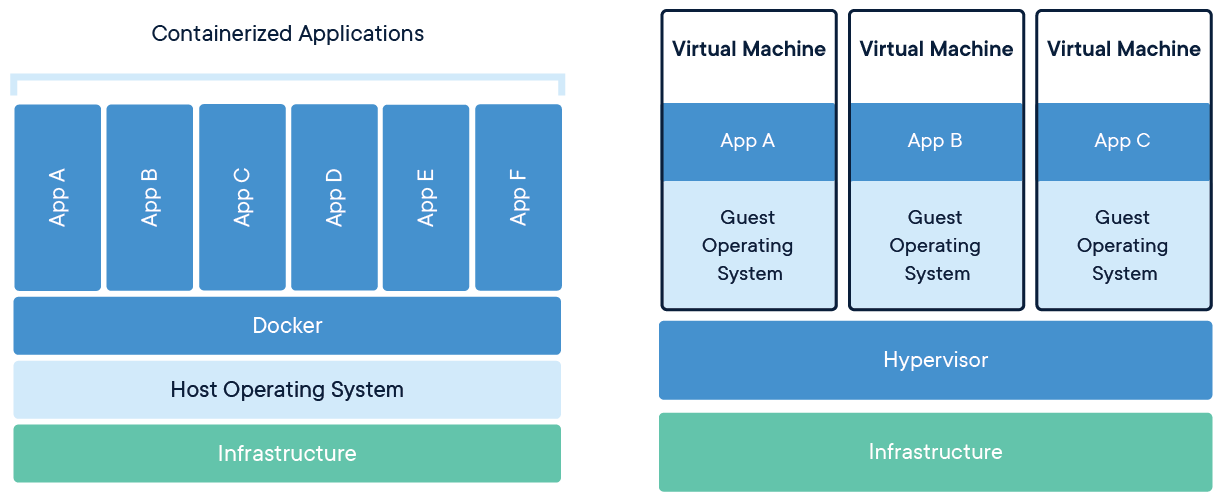
\includegraphics[width=1\textwidth]{images/docker-containerized-and-vm-transparent-bg.png}
				\caption{Docker Virtualisierung verglichen mit virtuellen Maschinen \cite{DockerInc..2020}}
				\label{fig:dockerComparison}
			\end{figure} 
			
			\subsubsection{DockerHub}		
				
				Eine Platform, die ebenfalls von Docker Inc. bereitgestellt wird, ist der sog. DockerHub. Dieser stellt eine Registry für Docker Images und Repositories dar und bietet dem Nutzer die Möglichkeit selbst erstellte Images hochzuladen und somit anderen Nutzern zur Verfügung zu stellen. 
				
				Ferner bietet Docker eine Versionsverwaltung, welche es ermöglicht verschiedene Versionen eines Images zu erstellen. So sind die verschiedenen Versionen eines Images auf dem DockerHub einsehbar.
		
		\subsection{Android}
		
			\subsection{Kotlin}
		
	\section{Qualitätssichernde Maßnahmen}
	
		\subsection{Code Review}
		
		% Git, Gerrit unso dies das
	
		\subsection{Continuous Integration}
		
		\subsection{Testing Frameworks}
		                                                                                                                                                                                                                                                                                                                                         
	
\chapter{Anforderungen}

(Joshua)

In diesem Kapitel sollen die Anforderungen an die zu erstellende Applikation beschrieben werden, um den zu erreichenden Scope festzulegen und eine abschließende Bewertung durchführen zu können, die das Erreichte mit den Zielen vergleicht.

\vspace{0.25cm}

Zuerst wird die Begrifflichkeit \enquote{Anforderung} geklärt. In der Softwareentwicklung gibt es einige verschiedene Definitionen von \enquote{Anforderungen}. In dieser Arbeit soll der Definition gefolgt werden, welche von Helmut Balzert in seinem Buch zu den Basiskonzepten und des Requirements Engineering erarbeitet wurden \cite{Balzert.2009}. In seinem Werk werden Anforderungen wie folgt definiert.

\begin{defStrich}[Anforderungen]
	\enquote{Anforderungen (requirements) legen fest, was man von einem Definition
		Softwaresystem als Eigenschaften erwartet.} Mit der Annahme, dass \enquote{man} alle Stakeholder (Personen, die ein Interesse an der Entwicklung und/oder der erstellten Software haben) beinhaltet. \cite{Balzert.2009}
\end{defStrich} 

Des Weiteren sollten vor der Festlegung der Anforderungen \enquote{Visionen und Ziele} und die Rahmenbedingungen, in denen die Software existieren sollen, festgelegt werden. Erst danach sollten Eigenschaften, welche in \enquote{funktionale} und \enquote{nichtfunktionale} Eigenschaften unterteilt werden können, definiert werden. In den folgenden Unterkapiteln wird nach diesem Prinzip vorgegangen, um eine konsistente und sinnvolle Anforderungslage zu schaffen.

\section{Visionen und Ziele}
An erster Stelle der Anforderungen steht eine Vision für das zu erstellende Produkt. In diesem Fall wurden bereits einige wichtige Punkte in der Einleitung der Arbeit zusammen gefasst, die zu einer kurzen und Prägnanten Vision führen:

\vspace{0.25cm}

\enquote{Durch \textit{Travlyn} sollen Nutzer in der Lage sein, ihre Städtereisen ohne das Mitführen von papierbasierten Reiseführern oder die Nutzung von multiplen mobilen Diensten zu bewältigen, ohne dabei einen Informationsverlust oder eine Beeinträchtigung des Reisespaßes hinnehmen zu müssen.}

\vspace{0.25cm}

Anhand dieser Version, die beschreibt, was erreicht werden soll aber nicht wie, werden konkrete Ziele abgeleitet. Es wurde entschieden, dass diese Ziele dem \enquote{SMART} Prinzip folgen sollten.

\begin{defStrich}[SMART Ziele]
	Die Art und Weise messbare Ziele zu setzen kann einer festgelegten Struktur folgen. In diesem Fall soll die Struktur, welche Peter Drucker in seinem Buch \enquote{The Practice of Management} (1954) erarbeitet hat, genutzt werden. Allerdings hat Drucker nie eine genaue Erklärung zu der Bedeutung des Akronyms \enquote{SMART} abgegeben, deswegen wird folgende allgemein akzeptierte Vaiante gewählt\cite{Lawlor.2012}:
	\begin{itemize}
		\item Specific (Spezifisch)
		\item Measurable (Messbar)
		\item Attainable (Erreichbar)
		\item Realistic (Realistisch)
		\item Timely (Rechtzeitig)
	\end{itemize}   
\end{defStrich} 

Folgend diesem Prinzip sind folgende Ziele entstanden:

\begin{itemize}
	\item Ein Nutzer soll sich vor einer Reise über \textit{Travlyn} folgende Informationen zu seiner Zielstadt einholen können: Name, Lage, Beschreibung und ein Bild, welches einen ersten Eindruck der Stadt vermittelt.
	\item Vor und während der Reise wird \textit{Travlyn} den Nutzer entlang einer vorher festlegten Route durch die Stadt leiten und Informationen, wie Beschreibungen, Bilder und Kosten anzeigen.
	\item Während der Führung durch \textit{Travlyn} werden einzelne Texte per machine learning zu einer zusammenhängenden Führung zusammengefasst und von Android vorgelesen um den Eindruck eines realen Guides zu schaffen.  
\end{itemize}

\section{Rahmenbedingungen}
Laut Balzert stellen Rahmenbedingungen \enquote{organisatorische und/oder technische Restriktionen für das Softwaresystem und/oder den Entwicklungsprozess} da \cite{Balzert.2009}.

\subsection{Organisatorisches}
Für \enquote{Travyln} liegen folgende organisatorische Rahmenbedingungen vor: Der Anwendungsbereich der Software liegt im privaten Umfeld, genauer gesagt im Bereich des privaten Reisens. Die Zielgruppe sind alle Personen, die für relativ kurze Zeiträume in größere Städte reisen und diese mit ihren Sehenswürdigkeiten entdecken wollen und sich zu diesen weiter informieren wollen. Damit liegt eine mobile Benutzung unter ständiger Beobachtung des Nutzers vor. Während der Reise/der durch \textit{Travyln} geführten Tour wird die Anwendung ohne Unterbrechung laufen.

\subsection{Technisches}

Die technischen Anforderungen werden an dieser Stelle in zwei Abschnitte aufgeteilt, da sich die Rahmenbedingungen für den Server und den Client stark unterscheiden. 

\vspace{0.25cm}

Für den Server wird festgelegt, dass er in einem Docker-Container\cite{TODO} läuft, welcher unabhängig von dem darunterliegendem Betriebssystem ist. Peripherie wird es an diesem Rechner keine geben, da er nur per remote Zugriff von außen gesteuert werden wird. Die wichtigste Rahmenbedingung ist, dass die Hardware auf der der Server läuft ständig mit dem Internet verbunden sein muss, um eine dauerhafte Verfügbarkeit zu gewährleisten

\vspace{0.25cm}

Für den Client wird festgelegt, dass er auf einem mobilen Smartphone, welches im Akkubetrieb operiert, läuft. Auf dem Gerät muss Android als Betriebssystem laufen und die Version soll 7.0.0 (TODO) nicht unterschreiten. Das Gerät stellt eine klassische mobile Peripherie zur Verfügung, welche z.B. eine virtuelle Tastatur, einen GPS-Sensor und einen Lautsprecher/Kopfhöreranschluss beinhaltet. Auch für den Client muss eine konstante Internetverbindung existieren, um sicher zu stellen, dass der Server ständig erreicht werden kann und die entsprechenden Informationen abgefragt werden können.

\section{Geforderte Eigenschaften}
Nachdem die Ziele und die Rahmenbedingungen definiert sind, können die erwarteten Eigenschaften erarbeitet werden. Bei jeder Eigenschaft sollte geprüft werden, ob diese im Sinne eines der gesteckten Ziele sind und zum Erreichen der Vision beitragen und ob diese im Sinne der Rahmenbedingungen erreichbar und realistisch ist. Wenn eine dieser beiden Prüfungen nicht positiv erfüllt wird sollte über eine Redefinition der Eigenschaft nachgedacht werden, denn in der aktuellen Form ist sie nicht zielführend und kann mit dem vorliegendem Rahmen ggf. nicht umgesetzt werden.

\vspace{0.25cm}

Wie im vorherigen Verlauf beschreiben werden Eigenschaften häufig in \enquote{funktional} und \enquote{nicht-funktional} aufgeteilt \cite{Balzert.2009}. Im Folgenden wird dieser Trennung gefolgt.

\subsection{Funktionale Eigenschaften}
Unter funktionalen Eigenschaften wird alles spezifiziert, was ein System tun und explizit nicht tun/können soll. Laut Balzert können diese Eigenschaften in statische, dynamische und logische Eigenschaften aufgeteilt werden\cite{Balzert.2009}. Wir haben uns explizit gegen eine solche Gliederung entschieden, um einen zu großen Mehraufwand zu sparen und den Rahmen dieses Kapitels nicht zu sprengen.

\vspace{0.25cm}

Zur Visualisierung der erwarteten funktionalen Eigenschaften wurde ein Use Case Diagramm erstellt.
\begin{figure}[H]
	\centering
	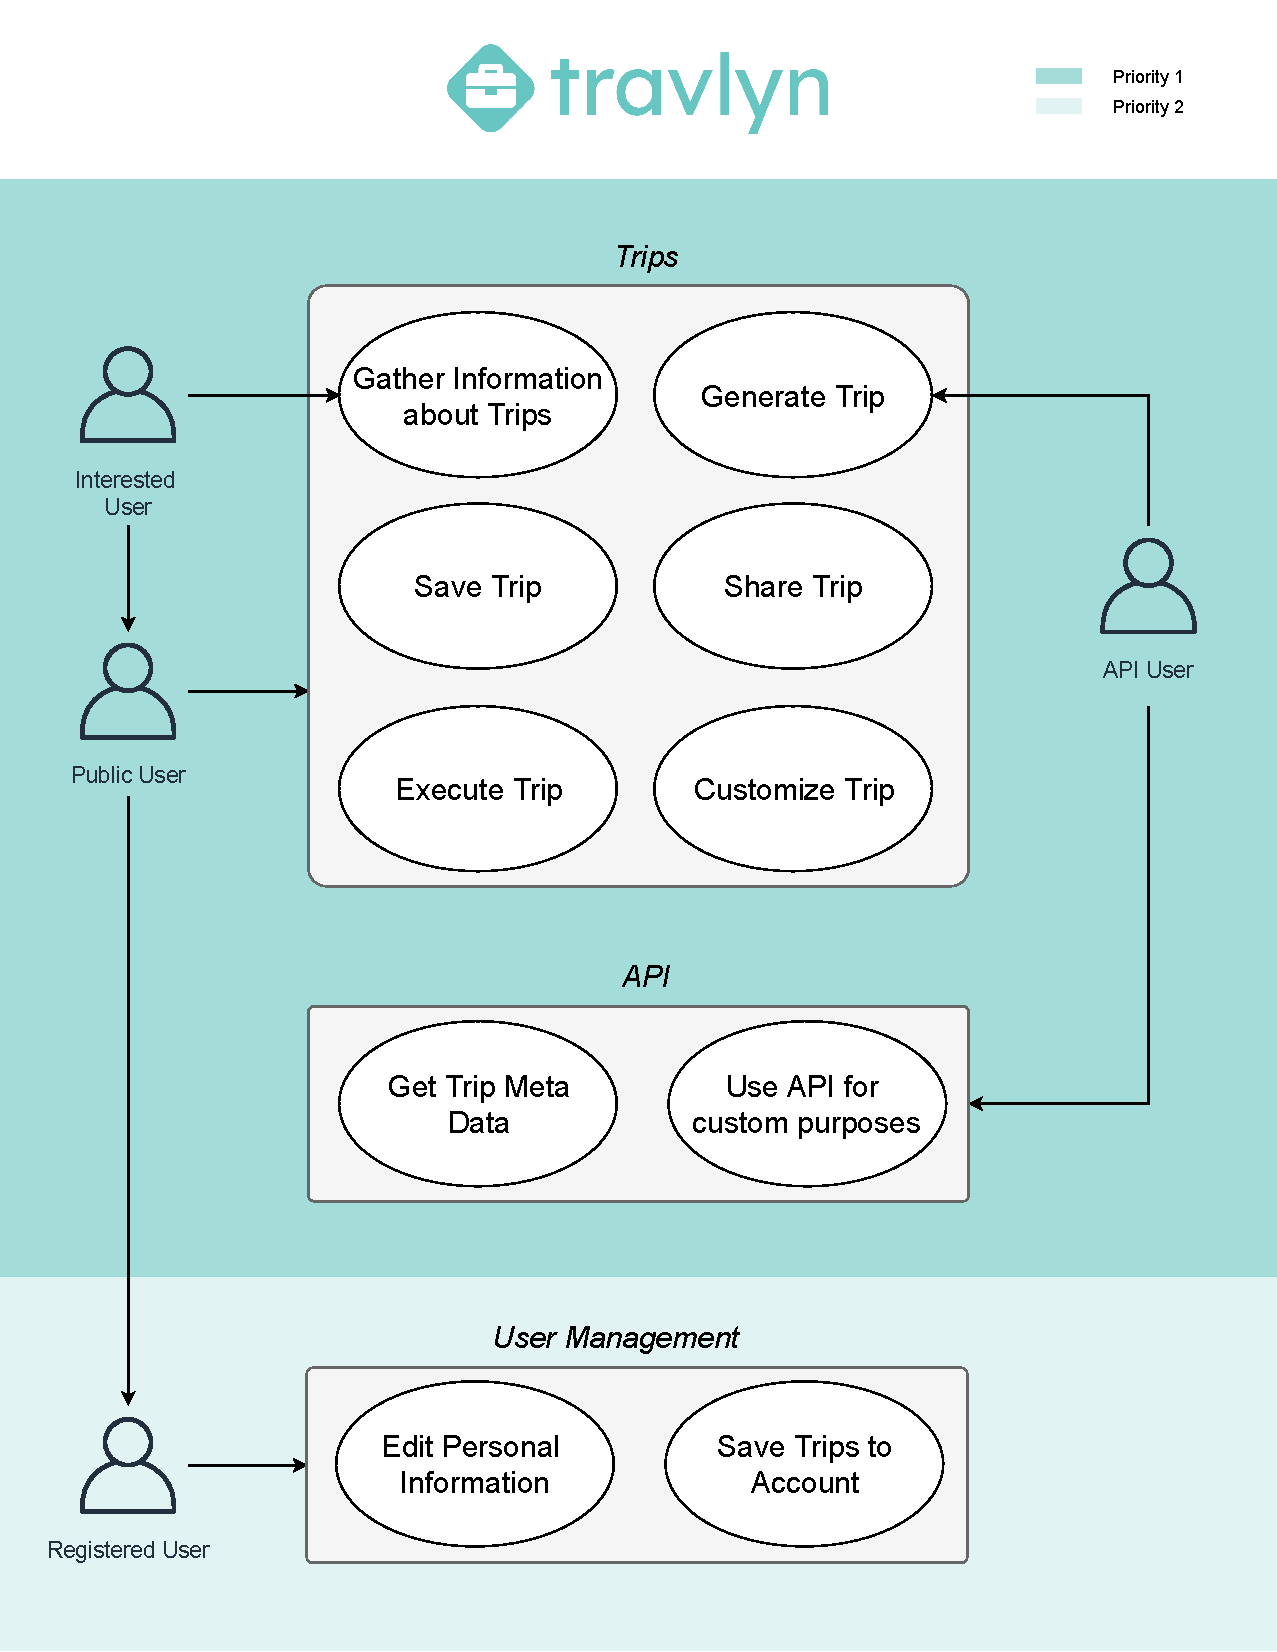
\includegraphics[width=1\textwidth]{images/UCD.pdf}
	\caption{Darstellung aller geplanten use cases mit den assoziierten Nutzerprofilen.}
	\label{fig:UCD}
\end{figure}

\newpage

Alle in \autoref{fig:UCD} dargestellten use cases wurden auf ihre Kompatibilität zu Zielen und Rahmenbedingungen geprüft und für passend befunden. Zusätzlich wurden sie bereits grob priorisiert. Es ist wichtig zu erwähnen, dass viele der dargestellten use cases im Laufe der Entwicklung zu kleinen Einheiten aufteilt werden, die hier im Sinne der Übersichtlichkeit nicht dargestellt sind.

Abschließend ist zu erwähnen, dass die funktionalen Anforderungen der in der Einführung geschilderten Funktionalität folgen soll.

\subsection{Non-Funktionale Eigenschaften}
Neben den geschilderten funktionalen Eigenschaften gibt es weitere Anforderungen, welche sich nicht direkt auf die Funktionalität und den Funktionalitätsumfang auswirken. Diese Eigenschaften werden auch \enquote{Quality of Service} (QoS) genannt und beinhalten häufig Eigenschaften wie  Genauigkeit, Verfügbarkeit und  Konsumierbarkeit. Es ist zu erwähnen, dass einige dieser Anforderungen miteinander in Konflikt stehen und ein geeigneter Mittelweg gefunden werden muss z.B. bestimmte Trade-offs eingegangen werden müssen, z.B. schränkt die Eigenschaft der möglichst hohen Sicherheit meist die Eigenschaft der Benutzbarkeit oder der Speichereffizienz ein \cite{Balzert.2009}.  

\vspace{0.25cm}

Für diese Softwareentwicklung soll für die non-funktionalen Eigenschaften als Orientierung die internationale ISO/IEC 25010 Norm gelten. Diese Norm setzt Standards für die Qualitätskriterien und -bewertung von Software und ist in drei Bereiche aufgeteilt\cite{ISO.2011} \cite{Braun.2016}:

\begin{itemize}
	\item \textbf{Quality In Use Model}: Dieser Teil beschreibt alle Merkmale, welche die Interaktion zwischen Mensch und System beschreiben, wie z.B. Effektivität und Freiheit von Risiken.
	\item \textbf{Product Qualitiy Model}: Der zweite Teil der Norm beschreibt acht Charakteristiken, welche ein Softwareprodukt erfüllen sollte, u.a. Wartbarkeit, Sicherheit und Benutzbarkeit.
	\item \textbf{Data Quality Model}: Der dritte und letzte Teil beschreibt Ansprüche, welche an das Datenmodel gestellt werden sollten um eine möglichst konsistente Benutzung der Daten zu ermöglichen.
\end{itemize}

Diese Norm ist sehr umfangreich und für ein Studienprojekt nicht vollständig umsetzbar, ohne den Zeit- und Aufwandsrahmen zu sprengen, deshalb wurde einige wichtige Punkte heraus gefiltert auf die ein besonderes Augenmerk gelegt werden soll. Zusätzlich wurden einige themenspezifische Anforderungen hinzugefügt. Daraus ergibt sich folgende Liste:

\begin{itemize}
	\item \textbf{Benutzbarkeit}: Durch die intensive mobile Benutzung der \textit{Travyln} App sollte diese für alle gängigen Gerätetypen eine gute Nutzungserfahrung bieten, die Nutzer überzeugen kann und die Reise angenehm verlaufen lässt. Explizit soll an dieser Stelle die Performance der Software genannt werden, welche bei anderen Applikationen häufig für eine schlechte Benutzbarkeit sorgt.
	\item \textbf{Sicherheit}: Der Schutz persönlicher Daten wir immer wichtiger und soll auch bei \textit{Travyln} nicht vernachlässigt werden.
	\item \textbf{Wartbarkeit}: Die Software sollte über die bereits beschriebenen qualitätssichernden Maßnahmen und durch eine entsprechende Architektur gut wart- und erweiterbar sein.
	\item \textbf{Datenquellen}: Da diese Software im Rahmen eines Studienprojekts mit sehr begrenzten Ressourcen erstellt wird, können keine kostenpflichtige Services eingebunden werden. Außerdem sollen schwierige Lizenzfragen vermieden werden, indem komplett auf Opensource Dienste gesetzt wird, bei denen die Nutzung der Daten vollständig erlaubt und frei ist. 
\end{itemize} 
\chapter{Datengrundlage}
(Joshua)

Die Datengrundlage ist für einen Reiseführer sehr wichtig, da der gesamte Sinn eines Reiseführers darauf basiert, Informationen aufzubereiten und an den Leser/Nutzer weiter zu geben. Aus diesem Grund wurden für diese Arbeit mehrere Datenquellen zu unterschiedlichen Themen herausgesucht und verglichen. Im Folgenden sollen diese Alternativen und die angestellten Überlegungen sowie die endgültige Entscheidung, welche Daten für \textit{travlyn} verwendet werden sollen, aufgezeigt.

\section{Points of Interest}
Travlyn soll laut Spezifikation Trips erstellen können, welche eine Abfolge von interessanten und sehenswerten Punkten in einer Stadt ist. Diese \ac{POI} sollen über ein \ac{API} in die App integriert werden. Folgende Anforderungen sind an die Informationen und die API gestellt:

\begin{itemize}
	\item Die abgefragten Daten sollten möglichst für einen kommerziellen Nutzen zugelassen sein, damit während der Entwicklung keine schwierigen Lizenzfragen auftreten können und ggf. höhere Datenvolumen durch Nachfragen erreicht werden können.
	\item Da diese Arbeit ein Studienprojekt ist, für welches sehr begrenzte Ressourcen zur Verfügung stehen sollte die API kostenfrei benutzbar sein.  
	\item Die API sollte Daten für möglichst viele Städte/Orte zur Verfügung stellen, damit \textit{travlyn} möglichst überall eingesetzt werden kann.
	\item Zu den einzelnen POIs sollten neben dem Namen und der Position weitere Daten wie Beschreibungen, Öffnungszeiten und ggf. Bilder bereitgestellt werden.
\end{itemize}

\subsection{Google Places API}
Google ist einer der größten Anbieter von Ortsbasierten Services/Diensten und stellt eine API für POIs zu Verfügung \cite{Google.01.02.2020}. Diese API hat sehr weit gefächerte Funktionen, die von einer einfachen Suche über ausführliche Details zu interessanten Orten bis hin zu \enquote{user check-in} an einzeln Orten reichen. Diese große Funktionalität wäre für \textit{travlyn} sehr wertvoll. Allerdings sind die Google APIs nicht frei zugänglich und die Anzahl der Requests ist u.U. stark eingeschränkt \cite{Singhal.2012}. Außerdem ist die Nutzung der erhaltenen Daten nur in Verbindung mit anderen von Google bereitgestellten Services erlaubt \cite{Google.02.12.2019}, somit wäre die ganze \textit{travlyn} Applikation an Google gebunden.  

\subsection{Openroute service}
Openroute service \cite{TheHeidelbergInstituteforGeoinformationTechnology.} wird vom Heidelberger Institut für Geoinformationstechnik angeboten. Es handelt sich um eine Crowd Sourced API, d.h. sie wird durch Benutzer über OpenStreetMap (OSM) \cite{OpenStreetMap.} gespeist und ist damit frei zugänglich. Durch die Nutzung von OSM ergibt sich der weitere Vorteil, dass die API für Orte weltweit nutzbar ist. Leider sind die gelieferten Informationen nicht sehr umfangreich und beinhalten häufig keine genauere Beschreibung und keine Bewertung o.Ä.. Weiterhin sind Crowd Sourced Informationen meist nicht offiziell verifiziert und könnten u.U. falsch sein. Die Beschränkungen für diese API sind relativ gering (500 POIs requests pro Tag), allerdings können diese auf Nachfrage erhöht werden (z.B. für Bildungszwecke).

\begin{defStrich}[Crowdsourcing]
	Beim Crowdsouring wird das Wissen, die Kreativität oder die Arbeitskraft der Masse ausgenutzt. Jeder leistet einen kleinen Teil und zusammen ergibt sich ein großes Ganzes. Typische Beispiele sind z.B. Wikipedia oder die Klassifikation von Daten zum Machine Learning. Allerdings können diese Daten von jedem bewusst oder unbewusst verfälscht werden und sie sind sehr schwer zu verifizieren \cite{Winkler.2009}. 
\end{defStrich}

\subsection{Foursquare}
Die Firma Foursquare bietet ebenfalls eine API an \cite{Foursquare.}, über die Informationen zu interessanten Orten gelesen werden können. Die API ist weltweit einsetzbar und liefert sehr viele Informationen zu einzelnen Orten, wie Ratings, kurze Beschreibungen oder Adressen von denen Bilder in der gewünschten Auflösung abgefragt werden können. Die Anzahl der möglichen Requests kann durch die Registrierung einer Kreditkarte (trotz der kostenlosen Nutzung) auf ca. 100.000 pro Tag gesteigert werden. Allerdings können die kostenfreien Varianten dieser API nicht für kommerzielle Zwecke genutzt werden und die abgefragten Daten dürfen nicht länger als 24 Stunden persistiert werden. 

\subsection{Evaluation der Alternativen}
Für das Projekt wurde aus den obigen Alternativen gewählt. Die endgültige Entscheidung fiel auf den OpenRoute service, da es für unser relativ kurzes Projekt ein sehr großes Risiko darstellt, dass langwierige Nachforschungen zu Lizenzfragen und erlaubten Einsatzmöglichkeiten angestellt müssen. Openroute service ist selbst für kommerziellen Nutzen freigegeben und aus rechtlicher Perspektive damit sehr einfach zu nutzen. Im Gegensatz dazu stellen sowohl Google als auch Foursquare starke Einschränkungen auf, die ein nicht abzusehendes Risiko darstellen, z.B. sind bestimmte Funktionen unter diesen Einschränkungen umsetzbar. Trotz diesem entscheidenden Vorteil muss der Nachteil in Kauf genommen werden, dass nur mäßig ausführliche Informationen gelesen werden können. Im weiteren Verlauf dieser Arbeit werden weitere zusätzliche Datenquellen aufgezeigt, um diesen Nachteil möglichst gut aufzufangen.

\section{Weiterführende Informationen zu POIs und Städten}
Um die eingeschränkte API Openroute service auszugleichen und dem Nutzer weitere Informationen zu seinem Reiseziel und zu besuchenden Orten zu bieten müssen weitere APIs angefragt werden.

\vspace{0.25cm}

Die wahrscheinlich bekannteste und ausführlichste Datenquelle ist Wikipedia. Dies ist einen Crowd Sourced Enzyklopädie die von allen Nutzern gespeist werden kann. Aus diesem Grund ist die Nutzung direkt im Internet aber auch per API Zugriff kostenlos und frei nutzbar. Allerdings ist zu beachten, dass die enthaltenen Inforationen durch jeden verändert und ggf. gefälscht werden können und Wikipedia deshalb keine sichere Quelle für wissenschaftliche Arbeiten o.Ä. darstellt. Für den in dieser Arbeit vorliegenden Use Case wurde entscheiden, dass dieses Risiko annehmbar ist und der Vorteil der sehr großen Wissensbasis das Risiko überwiegen. 

\vspace{0.25cm}

Für den Zugriff auf Wikipedia gibt es unterschiedliche Möglichkeiten, im Folgenden werden zwei APIs beschreiben, die ausprobiert worden sind:

\begin{itemize}
	\item \textbf{MediaWiki}: Hinter Wikipedia und vielen anderen Wiki-Seiten steht die selbe Software: MediaWiki \cite{MediaWiki.24.01.2020}. Diese Software bietet eine sogenannte \textit{MediaWiki action API}, die viele Informationen zu allen Artikeln eines Wiki zurückliefern kann. Leider sind die Daten nicht über einen zentralen Aufruf abrufbar sondern es werden mehrere Abfragen in folge benötigt, um z.B. die URL eines der Bilder des Artikels zu ermitteln.
	\item \textbf{DBpedia}: Die zweite API, die mithilfe eines Protypes getestet wurde ist \textit{DBpedia} \cite{DBpedia.02.02.2020}. Auch diese API folgt dem crowd sourcing Prinzip und ist somit frei zugänglich. Zusätzlich können dort alle Informationen über einen zentralen Zugriff abgerufen werden, indem die benötigten Daten über URL-Parameter spezifiziert werden können. Außerdem bietet diese API die Daten in aufbereiteter Form an: Links können direkt aufgelöst werden, es wird das selbe Thumbnail ausgeliefert welches im original Artikel ausgewählt ist und es kann auf alle Daten der kompakten Infobox in der oberen rechten Ecke strukturiert zugegriffen werden.
\end{itemize}

Durch die einfachere Handhabung der \textit{DBpedia} API wurde für den weiteren Verlauf entschieden auf diese API zu setzen und alle Informationen zu POIs und Städten von diesem Zugang abzufragen. Damit können erweiterte Infos geladen werden, die dem Nutzer während seines Trips kontinuierlich angezeigt werden können, um die Erfahrung weiter zu verbessern.

\section{Kartendaten}

Neben den \acs{POI}s werden zur Aufbereitung der Informationen weitere Daten benötigt. Allen voran sind Kartendaten essenziell, um dem Nutzer Orientierung und eine Übersicht über die Lage der ausgewählten \acs{POI}s zu geben. Der \textit{Travlyn} Client soll auf Mobilgeräten laufen, im besonderen auf Android Geräten, wie in \autoref{sec:anforderungen} beschrieben. Aus diesem Grund muss ein Kartenformat gewählt werden, welches auf entsprechenden Geräten angezeigt werden und genutzt werden kann.

\vspace{0.25cm}

Auch bei diesem Thema stehen sich grundlegend zwei große Anbieter gegenüber: Google \cite{Google.01.02.2020} und OpenStreetMap \cite{OpenStreetMap.}. Aufgrund der ausführlichen Beschreibung im vorangegangenen Kapitel soll an dieser Stelle auf eine weitere Ausführung verzichtet werden. Auch bei dieser Entscheidung kann die Wahl nur auf OpenStreetMap fallen, da dies eine Crowd Sourced Datenbasis, welche größtenteils frei von Lizenzfragen in den meisten Umfeldern genutzt werden kann. Abgesehen vom Kostenfaktor ist dies der größte Vorteil gegenüber Services von Google, die allerdings meist im Funktionsumfang und der gebotenen Qualität überlegen sind.

\vspace{0.25cm}

Somit standen einige Android Dienste zur Auswahl, welche auf OpenStreetMap Karten operieren. Die Wahl fiel schlussendlich auf \textit{osmdroid}\cite{osmdroid.3162020}. Die Bibliothek \textit{osmdroid} kann als alternative zum Android MapView, welcher auf Google Karten operiert, genutzt werden. Sie bietet diverse Features wie offline Karten, Icons und selbst designbare Overlays. Besonders die Möglichkeit Karten auch offline anzeigen zu können bietet für die \textit{Travlyn} einen Vorteil, der ausgenutzt werden kann, wenn die Netzqualität unterwegs eher mäßig ist.

\vspace{0.25cm}

Die Bibliothek kann über \textit{Gradle} (siehe \autoref{sec:gradle}) eingebunden werden und ist damit leicht zu benutzen. Da diese Bibliothek Open Source ist und frei auf GitHub zur Verfügung steht, ist die Nutzung kostenfrei. Außerdem gibt es aktuell eine starke Weiterentwicklung und regelmäßige Releases. Hiervon versprechen wir uns bald weitere unter verbesserte Funktionen, die wir für \textit{Travlyn} nutzen können.
\chapter{Konzept}

(Joshua)

In diesem Kapitel soll beschrieben werden, wie die in \autoref{sec:frameworks} beschriebenen Frameworks und Technologien in diesem Projekt zusammen spielen sollen. Hierzu wird zum einen auf die Architektur des Servers, der die API zur Verfügung stellt, eingegangen und zum anderen beschrieben wie der mobile Client aufgebaut ist. Als letztes wird aufgezeigt, wie beide Applikationen miteinander kommunizieren.

	\section{Kommunikationsschema}
	Da bei diesem Projekt zwei unabhängige Applikationen entstehen (zum einen der mobile Client und zum anderen der Server), ist es sehr wichtig die Schnittstelle zwischen beiden möglichst früh festzulegen. Zudem ist es möglich aus der Beschreibung der Schnittstelle ein Code-Gerüst zu generieren, siehe \autoref{sec:swagger}. Aus diesen Gründen wurde entschieden mit dem Kommunikationsschema zu beginnen.
	
	\subsection{Entitäten}\label{sec:entities}
	
	Die entstandene Swagger Beschreibung der API beinhaltet die grundlegende Struktur der Entitäten, die in unserer Applikation genutzt werden sollen. Dazu zählen unter anderem:
	
	\begin{itemize}
		\item \textbf{Stop:} Die \acs{POI}s, die dem Nutzer angezeigt und zur Auswahl gestellt werden sollen werden in der Stop Entität gespeichert und kommuniziert. Diese Entität beinhaltet alle notwendigen Informationen, wie den Namen des interessanten Punktes, die geografische Lage und die Kategorie, welchem der Punkt zugeordnet ist. Des Weiteren sind Informationen zu Bewertungen enthalten, die von Nutzern abgegeben wurden. Damit bildet die Stopentität die Grundlage für einen \textit{Trip}, welcher aus einer Folge von \textit{Stops} aufgebaut ist. 
		
		\newpage
		
		\begin{figure}[ht!]
			\centering
			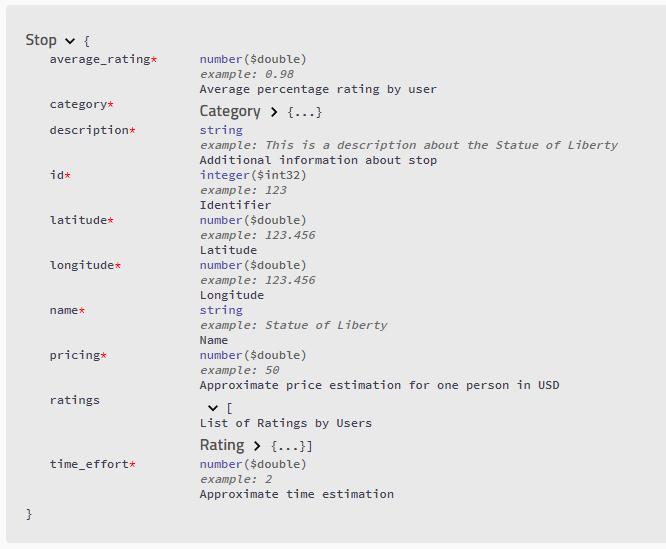
\includegraphics[width=1\textwidth]{images/swagger_stop_entity.png}
			\caption{Swaggerbeschreibung der Stopentität}
			\label{fig:swagger_stop}
		\end{figure} 
		
		\autoref{fig:swagger_stop} zeigt für die Stop Entität beispielhaft, wie eine Entitätsbeschreibung auf dem von Swagger bereitgestellten UI aussieht. Alle Elemente, die mit einem roten Stern gekennzeichnet sind, sind zwingend erforderlich um eine solche Entität anzulegen. Für jedes Attribut ist eindeutig festgelegt, welchen Typ es hat, ein Beispiel und eine kurze Beschreibung, welche die Benutzung erleichtern soll. Wie an den Attributen \textit{category} und \textit{ratings} zu erkennen, können die einzelnen Entitäten untereinander Verschachtelt werden, um eine konsistente und vollständige Typisierung zu erreichen.   
		\item \textbf{Trip:} Ein \textit{Trip} ist wie bereits erwähnt eine Abfolge von Stop Entitäten. Entsprechend ist der zentrale Bestandteil einer Trip Entität eine Sammlung von Stop Entiäten. Daneben gibt es weitere Informationen zu der zugeordneten Stadt, zum Veröffentlichungsstatus des Trips und zu ggf. vorliegenden Ratings.
		\item \textbf{City:} Jede Stadt, welche in \textit{Travlyn} besucht werden kann, wird in einer City Entität gespeichert. Diese Entität beinhaltet Informationen wie Name, Beschreibung und ein die Adresse eines aussagekräftigen Bildes der Stadt. Einer Stadt sind alle in dieser Stadt liegenden Trips zugeordnet. 
		\item \textbf{User:} Die User Entität beinhaltet alle klassischen Informationen zu einem Benutzer der App, dazu zählen z.B. seine E-Mail Adresse, seine technische ID und sein Name. Vor allem für das in  \autoref{sec:funcReq} beschriebene Nutzungsprofil \textit{Registered User} ist diese Entität von zentraler Bedeutung, da eine Identifizierung des Nutzers notwendig ist um Trips zu speichern oder persönlich zugeordnete Informationen anzulegen und zu verwalten.
	\end{itemize}

	Neben den hier beschriebenen Entitäten gibt es noch einige weitere kleinere Entitäten in diesem Projekt, wie z.B. das \textit{token} oder wie bereits in der Stop Entität verwendet das \textit{rating} und die \textit{category}. Diese Entitäten und alle genaueren Beschreibungen (wie \autoref{fig:swagger_stop}) sind im Sinne der Übersichtlichkeit nicht dargestellt, können aber bei Abruf der API eingesehen werden \footnote{\url{https://travlyn.raphael-muesseler.de/travlyn/travlyn/1.0.0/swagger-ui.html}}.
	
	\subsection{Requests}
	
	Neben den beschriebenen Entitäten beinhaltet die Swaggerbeschreibung Schemata, wie bestimmte Informationen von der API abgerufen werden können. Diese Beschreibung bietet jedem die Möglichkeit die API zu erkunden und schreibt damit genau vor, welche Services der Server bereitstellen muss aber auch wie der Client bestimmte Informationen erfragen kann.
	
	\vspace{0.25cm}
	
	Im Folgenden wird einer der Requests genauer beschreiben und die entsprechenden Elemente im von Swagger bereitgestellten UI gezeigt. Neben diesem beispielhaften Request gibt es viele weitere Requests mit unterschiedlichsten Spezifikationen, welche bei Bedarf auf der in \autoref{sec:entities} bereits beschriebenen Website Abgerufen werden können und sogar mit direktem Zugriff auf die implementierte API getestet werden können.
	\begin{itemize}
		\item \textbf{/stop/\{stopId\}:} Durch die Angabe einer technischen \textit{stopId} kann über diese Schnittstelle eine Stop Entität zu erfragen. Im Swagger UI wird der Request mit seiner Beschreibung und allen erforderlichen Parametern angezeigt.  
		
		\begin{figure}[ht!]
			\centering
			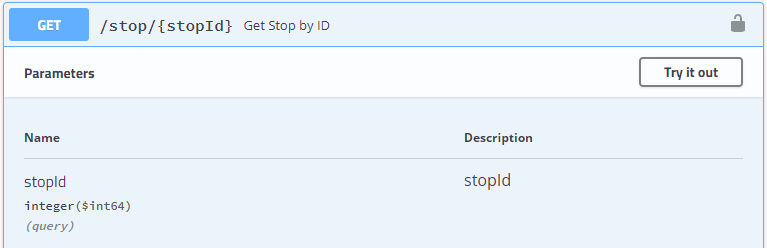
\includegraphics[width=1\textwidth]{images/swagger_getStop_head.png}
			\caption{Beschreibung des \textit{getStop} Requests im Swagger UI}
			\label{fig:swagger_getStop_head}
		\end{figure} 
		
		Außerdem werden die möglichen Antworten der API auf diesen Request angezeigt, um zu verdeutlichen was der Client genau zu erwarten hat und welche Fehler bei der Benutzung der Schnittstelle auftreten können.
		
		\begin{figure}[ht!]
			\centering
			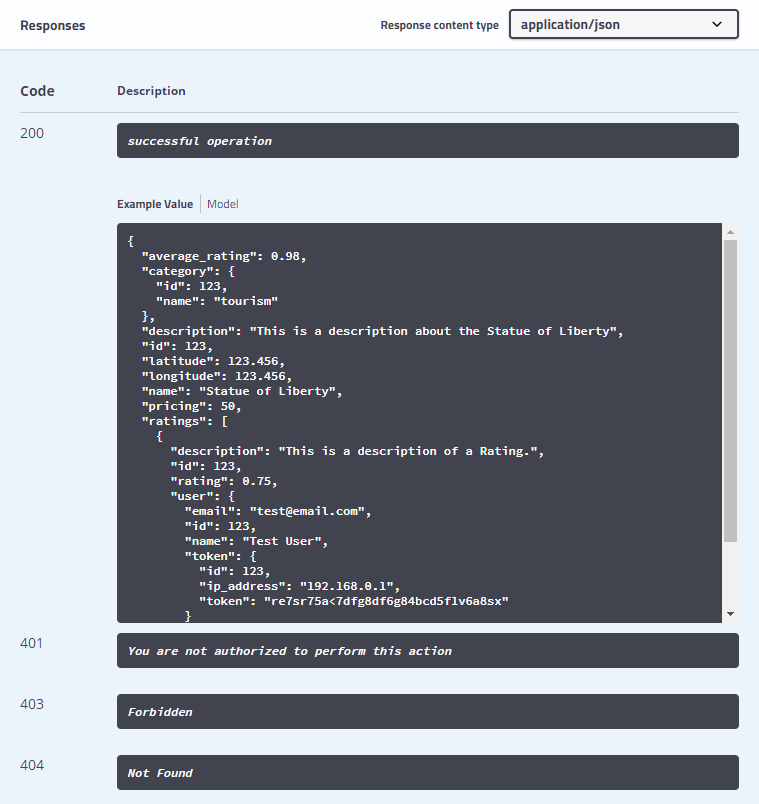
\includegraphics[width=1\textwidth]{images/swagger_getStop_response.png}
			\caption{Beschreibung des \textit{getStop} Requests im Swagger UI}
			\label{fig:swagger_getStop_response}
		\end{figure}
	
	Wie in \autoref{fig:swagger_getStop_response} zu sehen wird die Antwort im \acs{JSON} Format zurückgegeben, falls kein Fehler aufgetreten ist. In diesem Fall ist eine Antwort im selben Format zu erwarten, wie unter \enquote{Example Value} dargestellt. Dies ist die \acs{JSON} Darstellung der bereits vorgestellten Stop Entität (siehe \autoref{sec:entities}). Es sind alle Attribute, wie z.B. die Id oder der Name des \acs{POI}, wiederzuerkennen und in diesem Fall mit den gleichen Beispielwerten belegt, die in der Entitätsbeschreibung festgelegt wurden. Neben der erfolgreichen Antwort mit \acs{HTTP} Code 200 sind alle Fehlercodes, die von der API zurückgegeben werden können kurz beschreiben. Zusätzlich zu den hier gezeigten Codes ist der Code 500 (\textit{Internal Server Error}) zu berücksichtigen, welcher immer auftreten kann.
	
	\newpage
	
	\end{itemize}
		
	\section{Server Architektur}
	
	Wie in \autoref{sec:swagger} beschrieben ist es möglich aus der oben beschriebenen Swagger Beschreibung ein komplettes Code-Gerüst für eine Spring Applikation zu generieren. Diese Funktionalität wurde sich für das vorliegende Projekt zunutze gemacht. Damit entstand eine Spring Applikation, welche die in \autoref{sec:spring} beschriebenen Patterns verwendet und implementiert.
	
	\vspace{0.25cm}
	
	In \autoref{fig:UML} ist eine Übersicht über die grobe Struktur der Server Applikation zu sehen. Dieses UML Diagramm ist stark vereinfacht und beinhaltet nur beispielhafte Klassen, die symbolisch für einen größeren Verbund stehen sollen. So existiert wie bereits beschreiben nicht nur die Stop API und die dazugehörigen Interfaces und Klassen sondern noch viele weitere wie z.B. die User oder Trip API. Trotzdem ist erkennbar, dass sich die Serverarchitektur in mehrere Bereiche aufteilen lässt:
	
	\begin{itemize}
		\item \textbf{Spring-Klassen:} Zur Nutzung von Spring werden einige Klassen benötigt, um bestimmte Konfigurationen und Dienstprogramme aufzusetzen. Diese Klassen werden an sehr vielen Stellen über \textit{Dependency Injection} (siehe \autoref{sec:spring}) in Spring und andere Teile der Architektur eingebunden. Besonders hervorzuheben ist an dieser Stelle die Klasse \textit{TravlynServer}, welche die Methode enthält, um die komplette Springapplikation zu starten.
		\item \textbf{Controller:} Controller liegen ebenfalls unter starker Kontrolle des Spring Frameworks. Alle Requests, die auf der API eingehen werden von Spring an den entsprechenden Controller übergeben. Diese sind für die Verarbeitung der Anfragen verantwortlich und extrahieren Parameter, allerdings beinhalten sie keinerlei Businesslogik, sondern delegieren die Aufgaben an die zentrale Serviceklasse. Diese ist ebenfalls über \textit{Dependency Injection} eingebunden, um die Verwaltung der Beziehung dem Framework zu überlassen. Nach der Ausführung der Anfrage werden die entsprechenden Informationen zurückgegeben und für eine entsprechende \acs{HTTP}-Antwort gesorgt. Durch dieses Verfahren können serverinterne Informationen wie detaillierte Fehlernachrichten vor dem Nutzer der API versteckt werden, um Angriffe zu erschweren.
		
		Neben der funktionalen Bedeutung für die Anwendung beinhalten die Controller Dokumentation entsprechend zu der Swagger-Beschreibung. Diese sorgt dafür, dass die \textit{Travlyn} API selbständig von Nutzern erkundet werden kann.
		\item  \textbf{Service:} Die Klasse \textit{TravlynService} ist das Herzstück des Servers und beinhaltet die meiste Businesslogik. Sie steht zum Teil unter der Kontrolle des Spring Frameworks, muss aber komplett händisch implementiert werden. In dieser Klasse werden alle Operationen, die der Server ausführen muss (z.B. Login eines Nutzers, Sammeln der POI's für eine Stadt oder erzeugen eines Trips) implementiert. Diese Klasse hält alle anderen Komponenten, wie die Controller, den Datenbankzugriff und weitere externe Funktionalitäten zusammen und kontrolliert ihr zusammenwirken.
		\item  \textbf{DTOs und Entitäten:} Auf dem Server werden Objekte in zwei unterschiedlichen Formaten gehalten, welche nicht unter der Kontrolle vom Spring aber zum Teil unter der Kontrolle von Hibernate stehen. Zum einen existieren sog. \ac{DTO}s. Diese beinhalten ausschließlich die Inforationen, die als Ergebnis einer API-Abfrage übermittelt werden. Zum anderen sind Datenentitäten entstanden, wie sie von Hibernate genutzt werden. Die Entitäten besitzen die gleiche Struktur, wie die zugrundeliegenden Datenbanktabellen und damit alle vorliegende Informationen. Dieses Pattern wird genutzt um bestimmte Informationen zu verstecken und eine Trennung zwischen der Sicht des Servers auf die Daten und der Sicht des API Nutzers zu erreichen. In der Literatur wird dieses Pattern als \textit{Interface Segregation Principle} genannt und ist Teil des \textit{SOLID} Konzepts \cite{GOLL.2019}. Beide Objekttypen sind über entsprechende Methoden ineinander umwandelbar.
		\item \textbf{Hilfsklassen:} Neben allen bereits genannten Funktionalitäten müssen weitere externe Funktionen eingebunden werden. Im Fall von \textit{Travlyn} hauptsächlich fremde \acs{API}s, die alle nötigen Daten zu \acs{POI}s, Städten und Karten zur Verfügung stellen. Diese Zugriffe werden im Service benötigt, um die angefragten Operationen ausführen zu können. Dieser Teil der Applikation steht nicht unter der Kontrolle eines Frameworks und wurde händisch integriert. 
	\end{itemize}
	
	
	\begin{figure}[ht!]
		\centering
		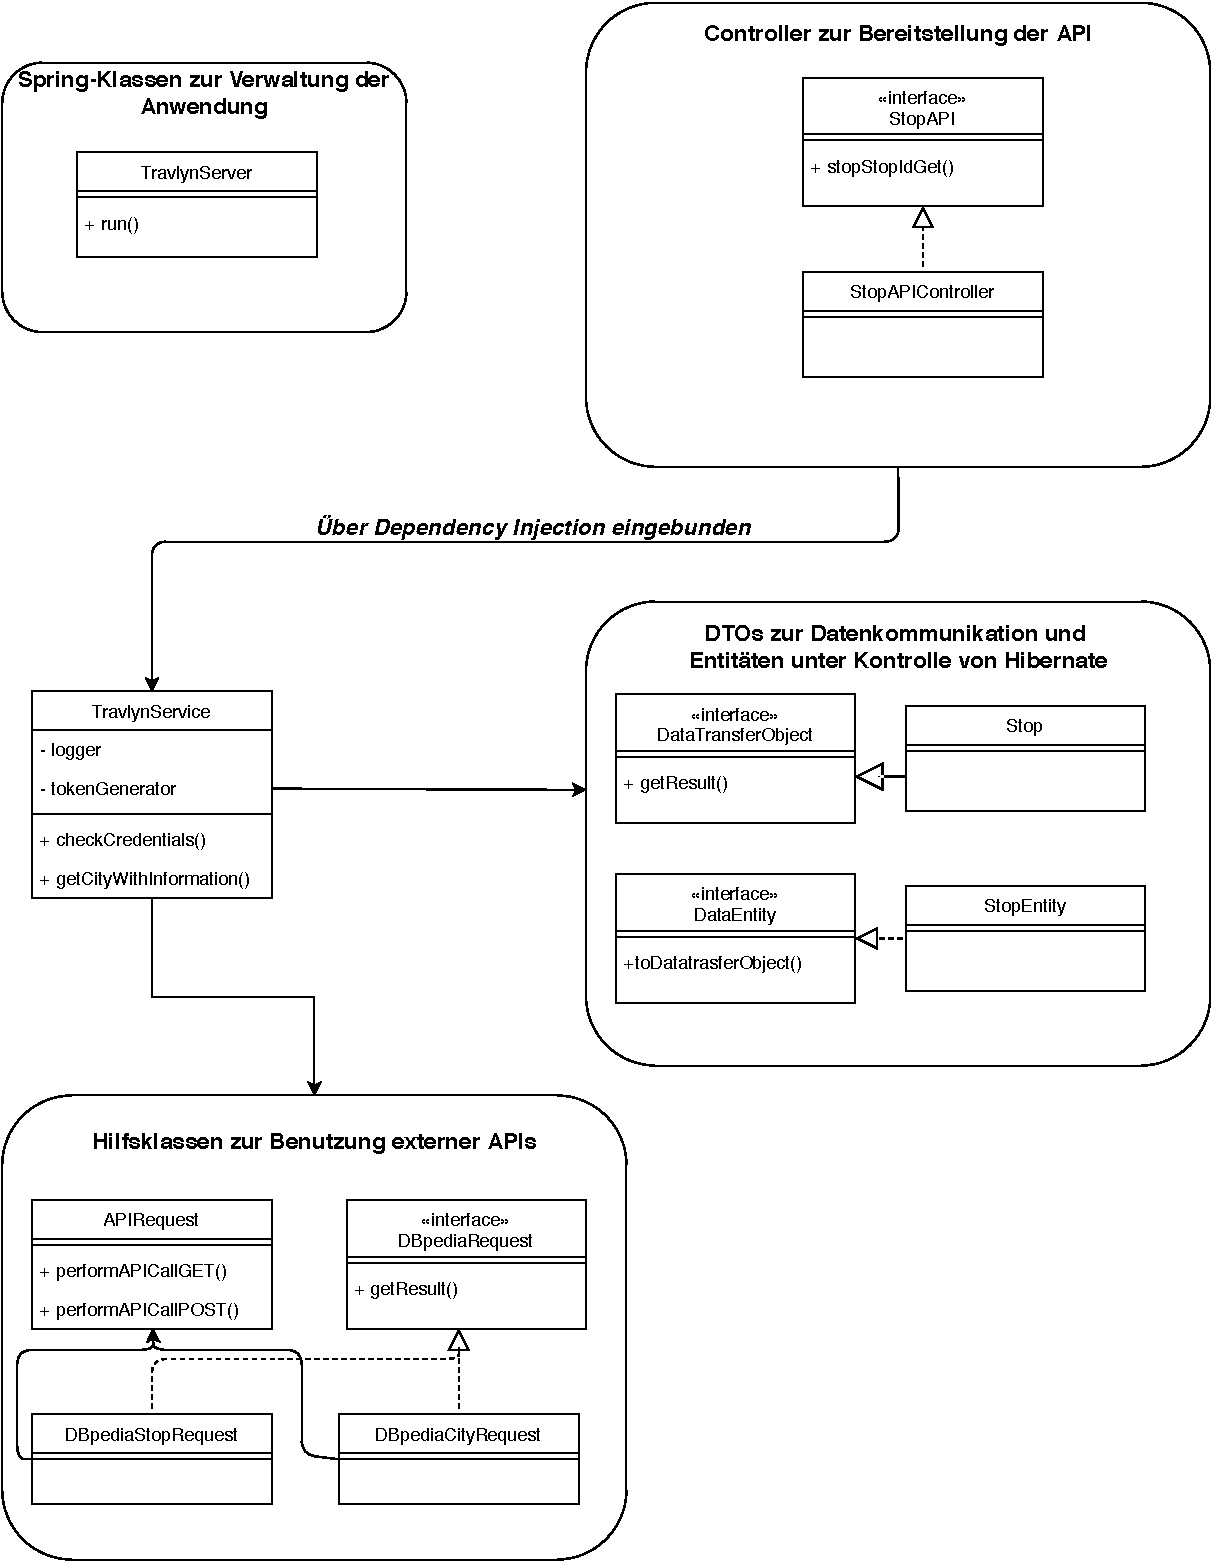
\includegraphics[width=1\textwidth]{images/UML_Diagram.pdf}
		\caption{Struktur des \textit{Travlyn} Servers als UML Diagramm. Zu Beachten ist, dass dieses Diagramm stark vereinfacht und nicht vollständig ist, um die Übersichtlichkeit zu wahren.}
		\label{fig:UML}
	\end{figure}

	\clearpage

	
	\section{Client Architektur}
		
		Neben der automatischen Generierung von Code, welcher das Spring Framework nutzt, ist es mit Swagger ebenfalls möglich, Code für den Client zu generieren. Da diese Generierung viel Arbeit und Einrichtungsaufwand spart, wurde auch das Grundgerüst für den \textit{Travlyn} Client automatisch generiert.
		
		\subsection{Model}
		
		\subsection{title}

	\section{Deployment Architektur}
	
		Wie bereits in \autoref{qm.continuous_delivery} wird der \textit{Travlyn} Server über ein Docker Image (siehe \autoref{frameworks.docker}) ausgeliefert. 
	
\chapter{Implementierung}

	In diesem Kapitel werden einige Implementationsdetails dargestellt und erläutert, welche entweder einen kritischen Aspekt des Projekts darstellen oder von hoher Relevanz für den Erfolg des Projektes sind. 
	
	\section{Controller Interfaces}
	
		Wie bereits erwähnt sind die sog. Controller in einer \acs{MVC} Architektur für den Behandlung von Benutzereingaben zuständig. Im Falle einer \acs{REST}ful \acs{API} -- hier durch Spring umgesetzt -- dienen Controller dem Zweck, alle eingehenden \acs{HTTP} Anfragen zu behandeln. Dafür bietet Spring Annotationen, mit dessen Hilfe eindeutig definiert werden kann, wie die Anfrage auszusehen hat. Diese Definition eines sog. Endpoints beinhaltet immer einen Pfad, unter welchem der Endpoint erreicht werden kann, und eine \acs{HTTP} Methode. Es kann zusätzlich noch festgelegt werden, welche \acs{HTTP} Header bei einer Anfrage angegeben werden sollen und welcher \acs{MIME} Type zurück gegeben wird.
		
		\autoref{code:CityApi} zeigt beispielhaft, wie eine solche Definition eines Endpoints aussehen kann. Die eigentliche Beschreibung des Endpoints wird durch die Annotation \lstinline|@GetMapping| beschrieben. 	
		
		Um jedoch eine ausführlichere Beschreibung des Endpoints zu erstellen, können die von Swagger bereitgestellten Annotation verwendet werden. So lassen sich beispielsweise die Parameter, die Rückgabewerte aber auch die Authentifizierungsmethode beschreiben. Außerdem lassen sich noch Beschreibungen einfügen, um die Benutzung der \acs{API} zu erleichtern und zu dokumentieren. Für die City \acs{API} wird ein String als Parameter benötigt, mit dessen Hilfe die entsprechende Stadt zurückgegebene werden kann. Außerdem wird ein \acs{API} Key benötigt, um sich zu authentifizieren. 
		
		\lstinputlisting[
			label=code:CityApi,
			caption=Nutzung der beschriebenen Annotationen eines Controllers am Beispiel der City API,
			captionpos=b,               % Position, an der die Caption angezeigt wird t(op) oder b(ottom)
			style=EigenerJavaStyle,     % Eigener Style der vor dem Dokument festgelegt wurde
		]{code/CityApi.java}
		
	\section{Authentifizierung}
	
		\begin{figure}[ht!]
			\centering
			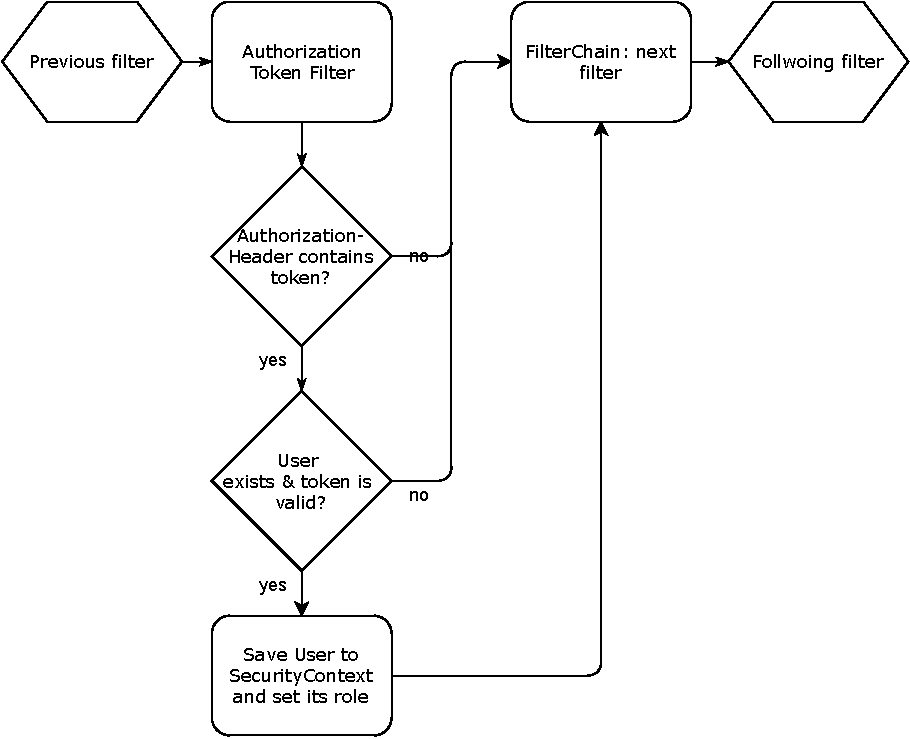
\includegraphics[width=1\textwidth]{images/authorization-flow-chart.pdf}
			\caption{Authentifizierungsprozess von \textit{Travlyn} mittels Spring Security Filter Chain}
			\label{fig:authenticationProcess}
		\end{figure} 
		
		\textit{Travlyn} stellt insgesamt zwei verschiedene Authentifizierungsrollen bereit. Wie \autoref{fig:UCD} zeigt, gibt es zum einen die Rolle des \acs{API}-Benutzers und die des registrierten Benutzers. Dem API Benutzer ist es erlaubt, Informationen wie beispielsweise über Trips anzufragen, wohingegen ein registrierter Benutzer auch die Möglichkeit hat, einen Trip zu erstellen. 
		
		Der Prozess der Authentifizierung basiert bei \textit{Travlyn} auf sog. Tokens. Sobald sich ein Benutzer registriert oder anmeldet, wird ein Token generiert -- das Token besteht aus 32 Zeichen und Ziffern und besitzt zudem ein Ablaufdatum, welches bei Überschreiten das Token als ungültig gekennzeichnet --, auf der Datenbank abgespeichert und zurück an den Benutzer gesendet. Um nun Endpoints anzufragen, welche eine Authentifizierung benötigen, wird dieses Token im \lstinline|Authorization|-Header im Format \lstinline|Bearer <token string>| gesendet. Auf dem Server erfolgt nun die Validierung des Tokens. So kann außerdem festgestellt werden, wer eine bestimmte Aktion ausgeführt hat. 
		
		Spring stellt für diesen Prozess einen Mechanismus bereit, um diese Authentifizierung möglichst einfach umzusetzen: Bevor eine Anfrage an einen bestimmten Endpoint zugelassen und die entsprechende Controller-Methode (wie bei \autoref{code:CityApi} beispielhaft gezeigt) aufgerufen wird, durchläuft diese Anfrage eine Reihe von Filtern. Diese sog. Filter Chain beinhaltet unter Anderem auch Authentifizierungsmechanismen, die sich eigens definieren lassen. So wurde für \textit{Travlyn} ein Filter namens \lstinline|AuthenticationTokenFilter| entwickelt, der dazu dient, das Token aus dem \acs{HTTP}-Header zu extrahieren und zu validieren. 
		
		Wenn das Token valide ist und auch der korrekten Benutzerrolle -- \acs{API}- oder registrierter Nutzer -- zugeordnet werden kann, wird die Anfrage an die entsprechende Controller Methode weitergeleitet und der entsprechende Nutzer im sog. \lstinline|SecurityContext| gespeichert, sodass auf die Rolle des Benutzers und auch auf den Benutzer selbst beim Prozessieren der Anfrage zugegriffen werden kann. Ist dies nicht der Fall, so wird diese Anfrage als nicht-authentifiziert markiert. \autoref{fig:authenticationProcess} visualisiert den Authentifizierungsprozess, wie er bei \textit{Travlyn} umgesetzt wurde.
		
		Um die zugelassenen Benutzerrollen für einen Endpoint der \acs{API} festzulegen, stellt das Modul Spring Security unter anderem die Annotation \lstinline|@PreAuthorize| zur Verfügung. Als Parameter wird ein in der \ac{SpEL} geschriebener Ausdruck übergeben, wie beispielsweise \lstinline|hasRole(API_USER)| in \autoref{code:CityApi}. So lässt sich die gesendete Authentisierung des Benutzers automatisiert überprüfen. 
		

\chapter{Evaluation}

(Joshua)

Die in dieser Arbeit vorgestellte \textit{Travlyn} Applikation wurde parallel zur Erstellung der schriftlichen Ausarbeitung entwickelt und enthält die in \autoref{sec:implementierung} dargestellten Feinheiten und Konzepte. Um den Erfolg dieser Entwicklung festzustellen, soll das erreichte Ergebnis gegen die Anforderungen aus \autoref{sec:anforderungen} validiert werden und festgestellt werden wie viele der Anforderungen erreicht werden konnten. Hierzu werden zuerst die einzelnen funktionalen und nicht-funktionalen Anforderungen mit dem Ergebnis verglichen, bevor die Erreichung der übergeordneten Ziele und Visionen bewertet wird. Dieses Kapitel wird in ein Fazit über die gesamte Arbeit und einen Ausblick über mögliche weitere Entwicklungen münden.

\section{Funktionale Anforderungen}\label{sec:funktional_evaluation}
Zuerst sollen die funktionalen Anforderungen betrachtet werden, welche in \autoref{sec:funktionale_eigenschaften} beschrieben sind. Diesen Anforderungen gegenüber stehen die in der Travlyn App implementierten Prozesse:

\begin{itemize}
	\item \textbf{User Management:} Nutzer können sich in der Travlyn App registrieren und eigene Informationen wie Name und E-Mail festlegen. Dadurch entsteht ein persistenter Account, mit dem sich die Nutzer im System anmelden können und nutzerbasierte Aktionen durchführen können, z.B. einen Trip anlegen oder Sehenswürdigkeiten oder Trips bewerten. Ebenso ist es möglich seine persönlichen Informationen zu bearbeiten und Präferenzen festzulegen, welche genutzt werden um die angezeigten Daten nach potentieller Attraktivität für den Nutzer zu priorisieren.
	
	
	\begin{figure}[ht!]
		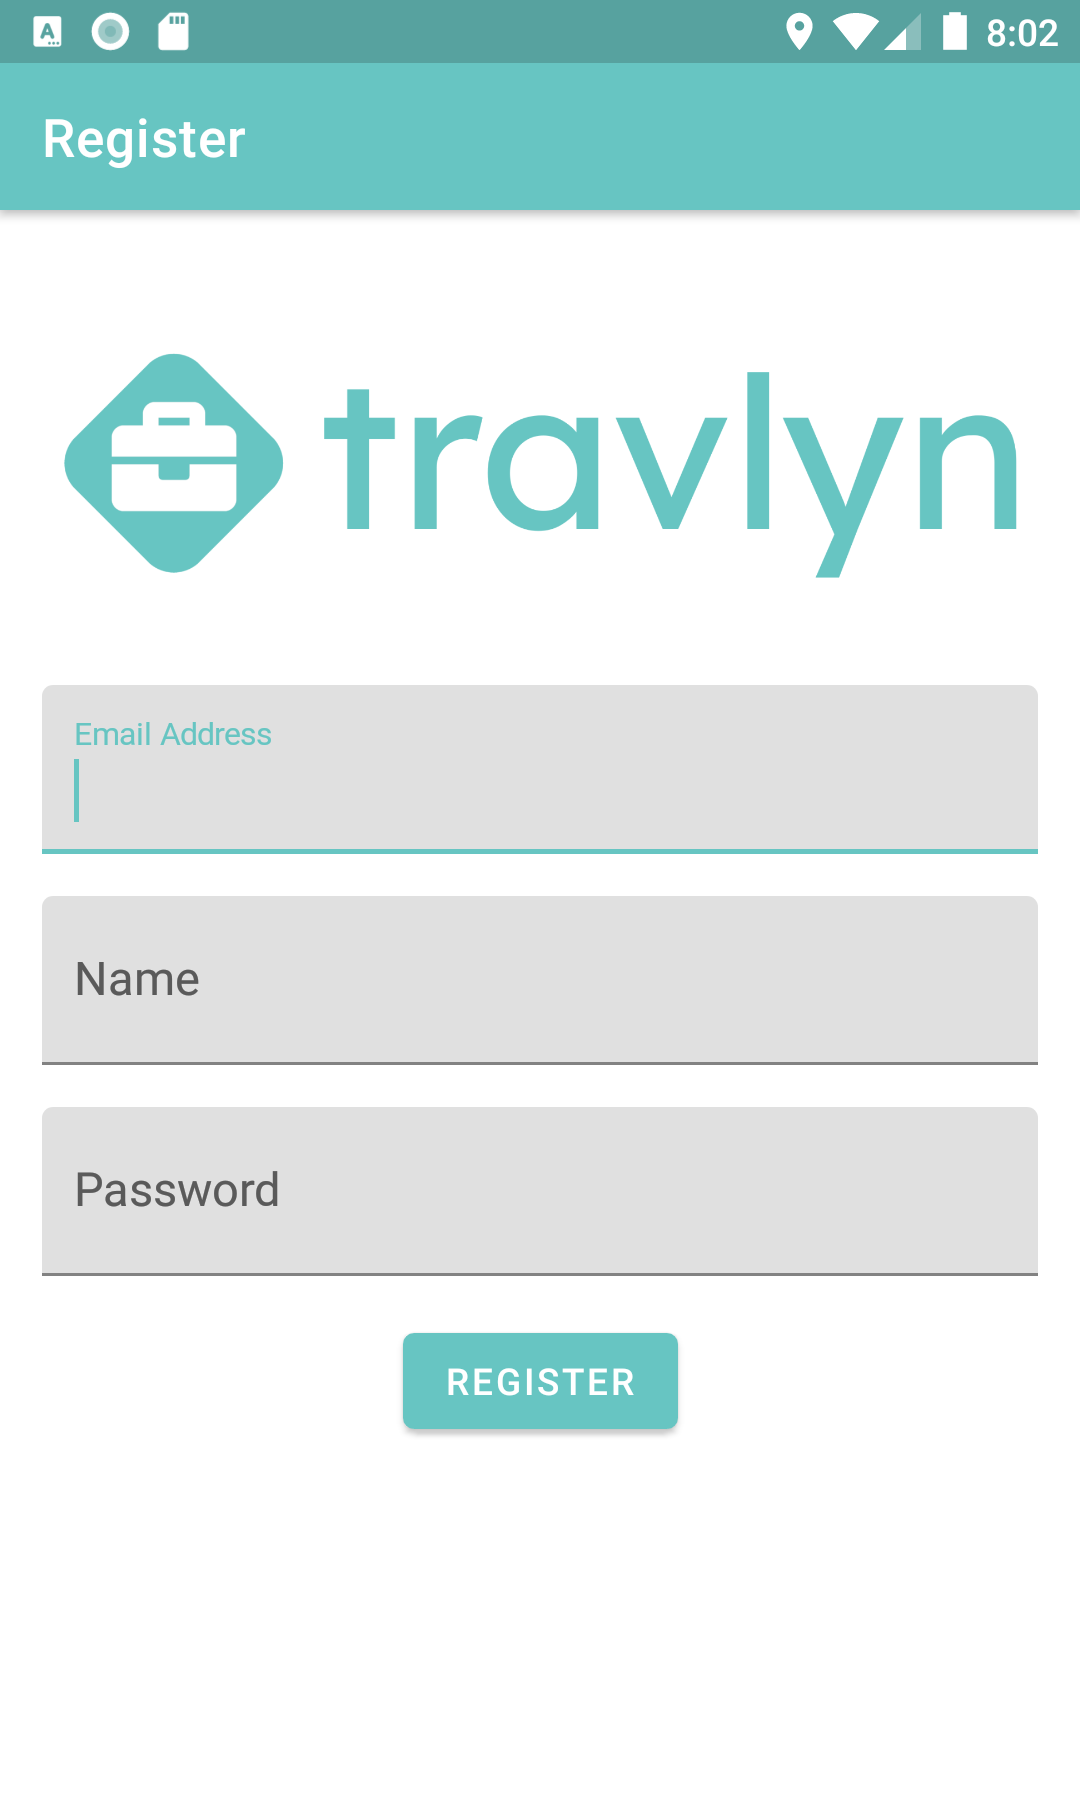
\includegraphics[width=0.32\textwidth]{images/travlyn-screenshot-register.png}
		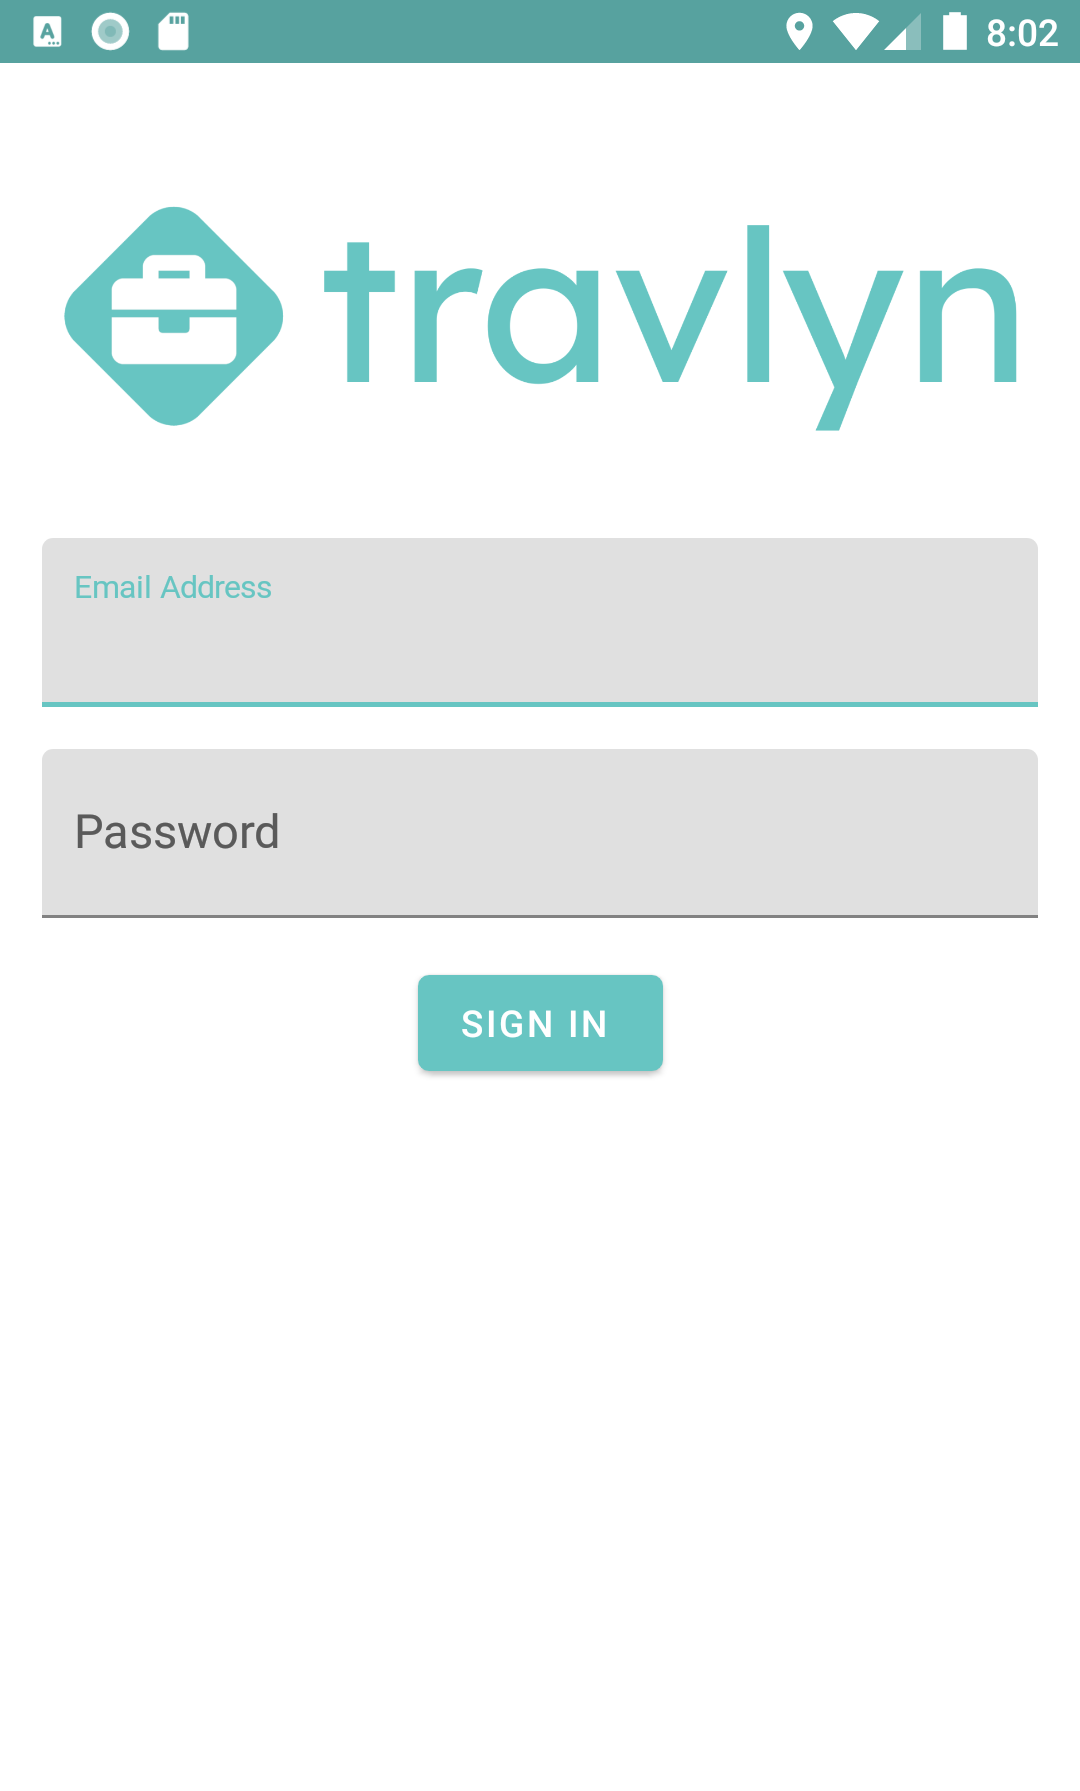
\includegraphics[width=0.32\textwidth]{images/travlyn-screenshot-login.png}
		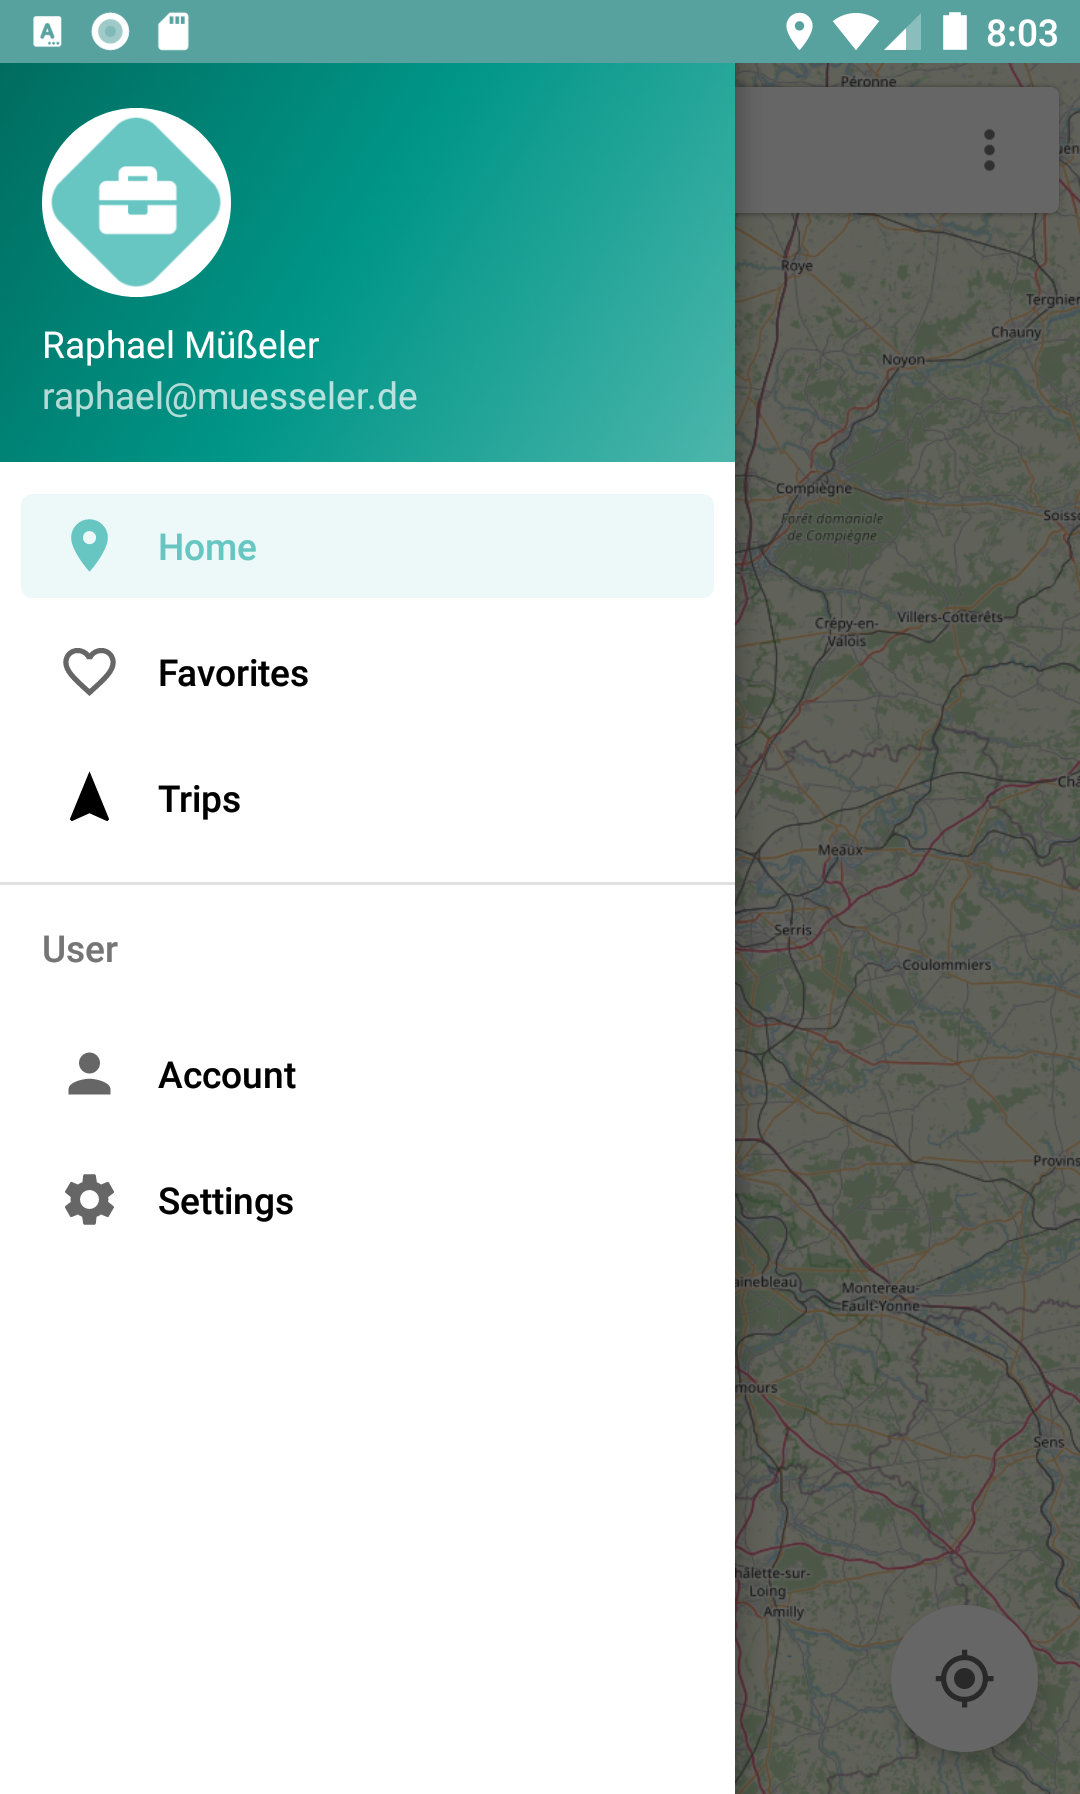
\includegraphics[width=0.32\textwidth]{images/travlyn-screenshot-side-navigation.png}
		\caption{User Management in der \textit{Travlyn} Applikation}
		\label{fig:ui_usermanagement}
	\end{figure}

	\newpage

 
	\item \textbf{Information über Städte:} In diesem Prozess kann ein Nutzer über die verfügbare Suchleiste nach jeder beliebigen Stadt auf der Welt suchen und erhält eine Beschreibung dieses Ortes. Falls es Sehenswürdigkeiten in direkter Nähe dieser Stadt gibt werden diese angezeigt und können in einer Detailliste mit ihren Metainformationen betrachtet werden. Außerdem werden ihm direkt die verfügbaren öffentlichen Trips angezeigt, welche für ihn ausführbar sind. Damit kann sich der Nutzer einen sehr vollständigen Eindruck einer Stadt verschaffen, welcher als Entscheidungsgrundlage für eine Reise dienen kann. Siehe \autoref{fig:ui_city_information}.
	
	\begin{figure}[ht!]
		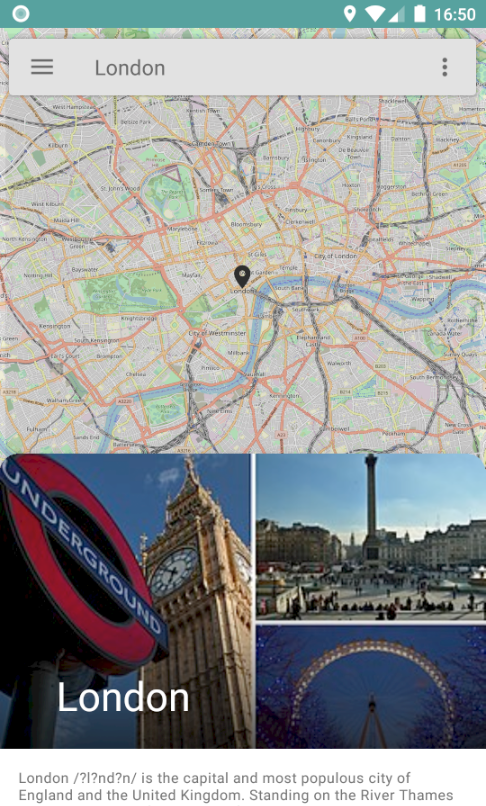
\includegraphics[width=0.32\textwidth]{images/travlyn-screenshot-search-result.png}
		
\includegraphics[width=0.32\textwidth]{images/travlyn-screenshot-city-detail.png}
		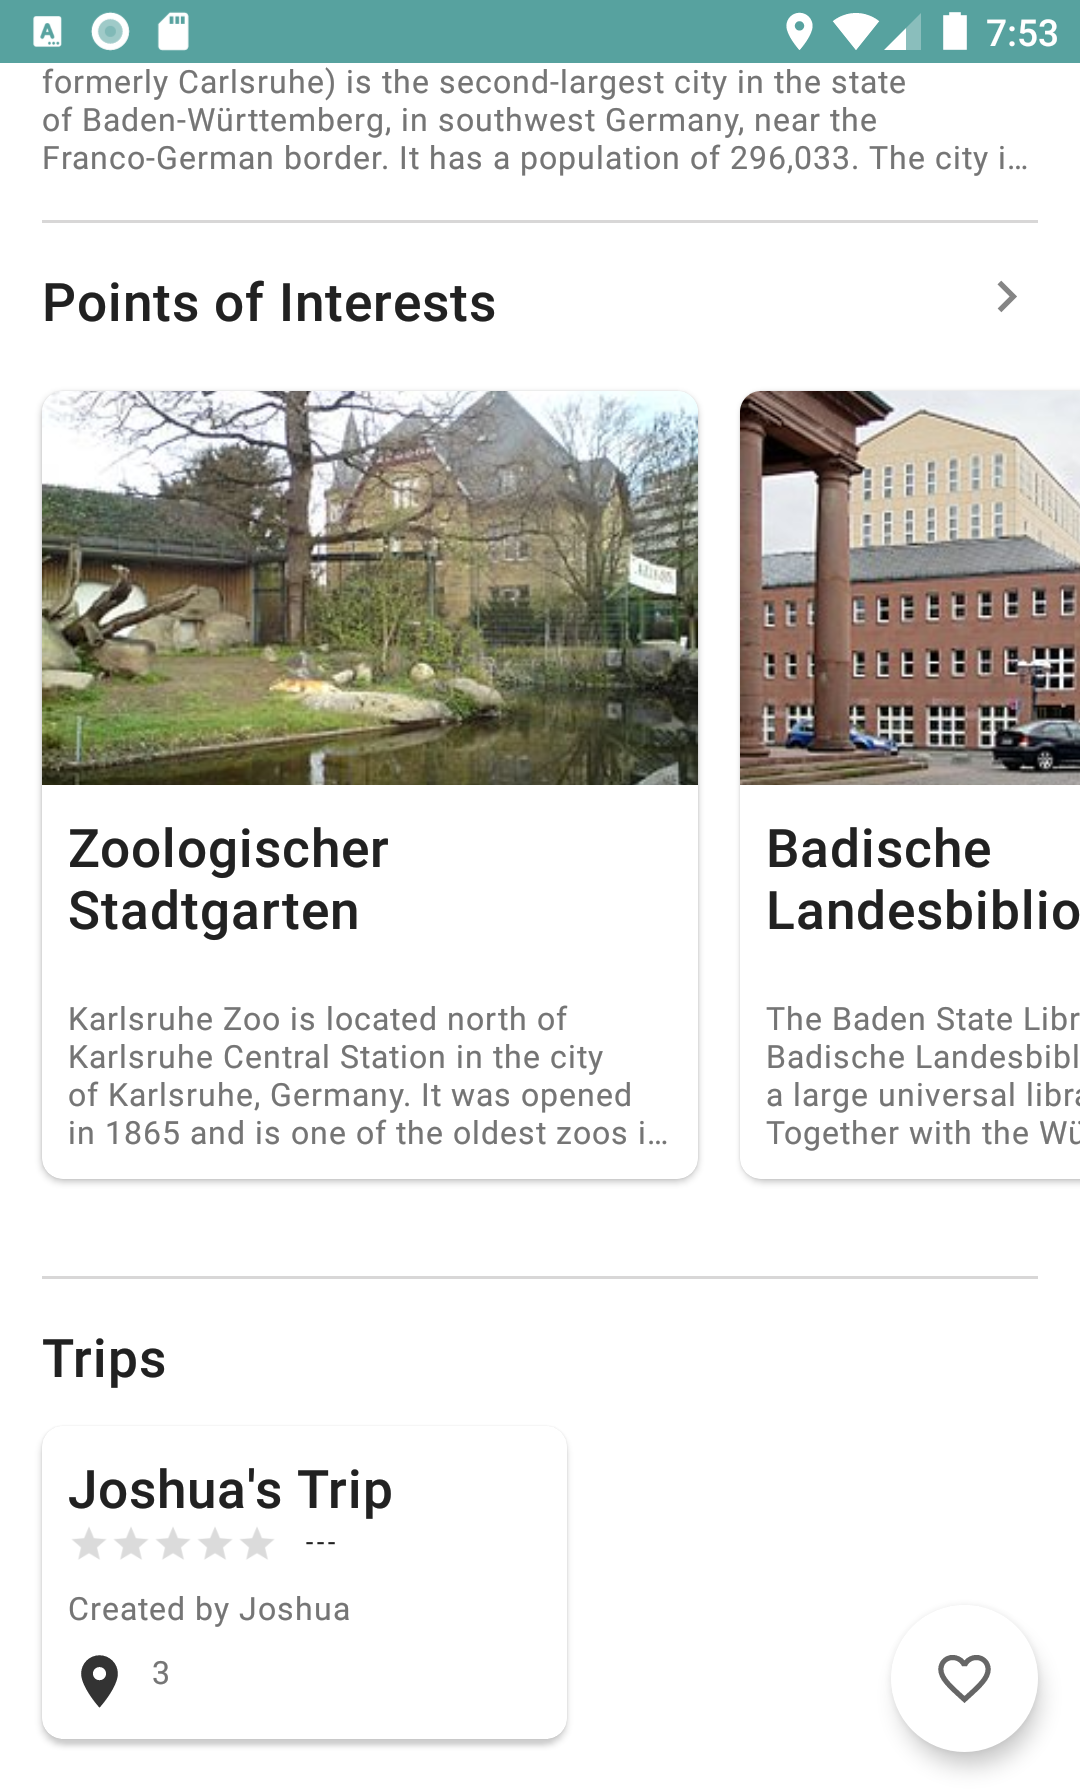
\includegraphics[width=0.32\textwidth]{images/travlyn-screenshot-city-detail-trips.png}
		\caption{Informationsangebot für eine gesuchte Stadt, in diesem Fall Karlsruhe}
		\label{fig:ui_city_information}
	\end{figure}


	\item \textbf{Trip Erstellung:} Ist eine konkrete Reise geplant, kann der Nutzer in der App einen Trip erstellen, welcher seine ausgewählten Sehenswürdigkeiten enthält und damit genau an den Umfang und Aufwand angepasst werden kann, den sich der Nutzer vorstellt. Es stehen ausnahmslos alle Ort und Kombinationen von Orten zur Verfügung. Nach der Auswahl und dem festlegen einiger Metainformationen ist der Trip direkt bereit zur Ausführung. Siehe \autoref{fig:ui_trip_creation}.
	
	\begin{figure}[ht!]
		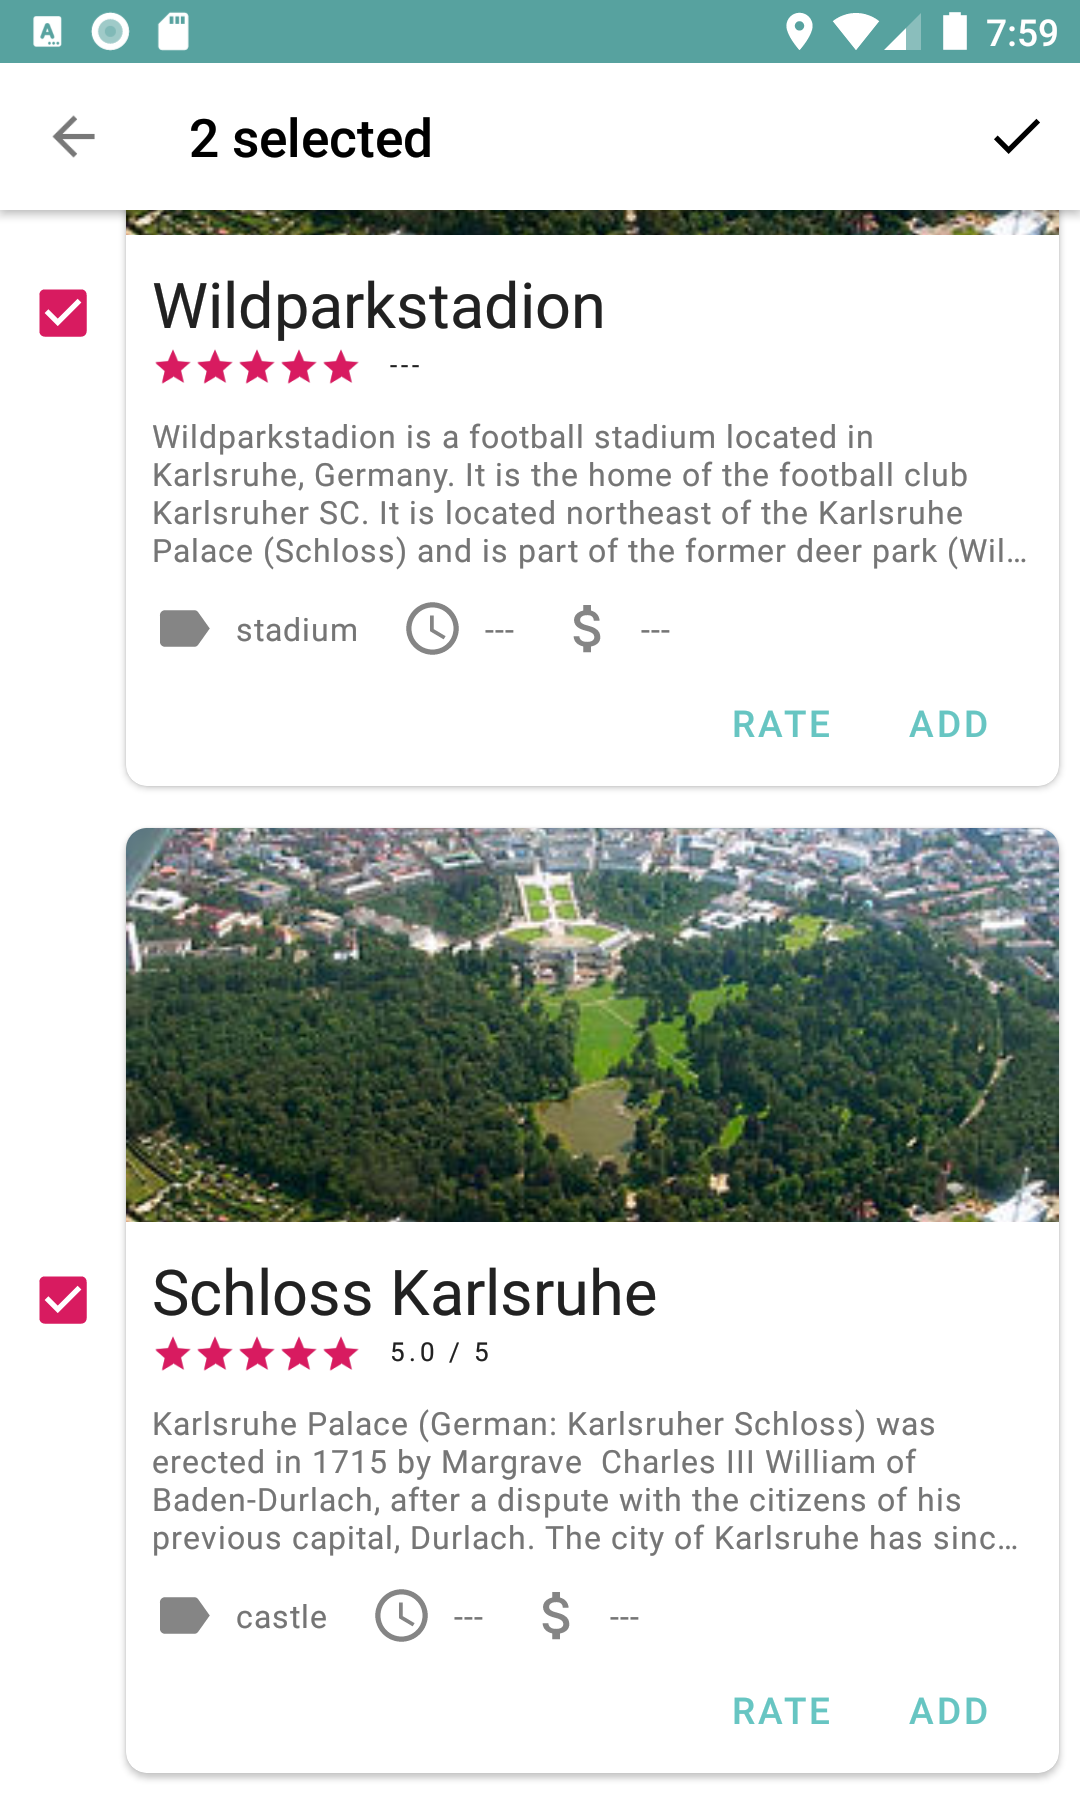
\includegraphics[width=0.32\textwidth]{images/travlyn-screenshot-stops-detail-selection.png}
		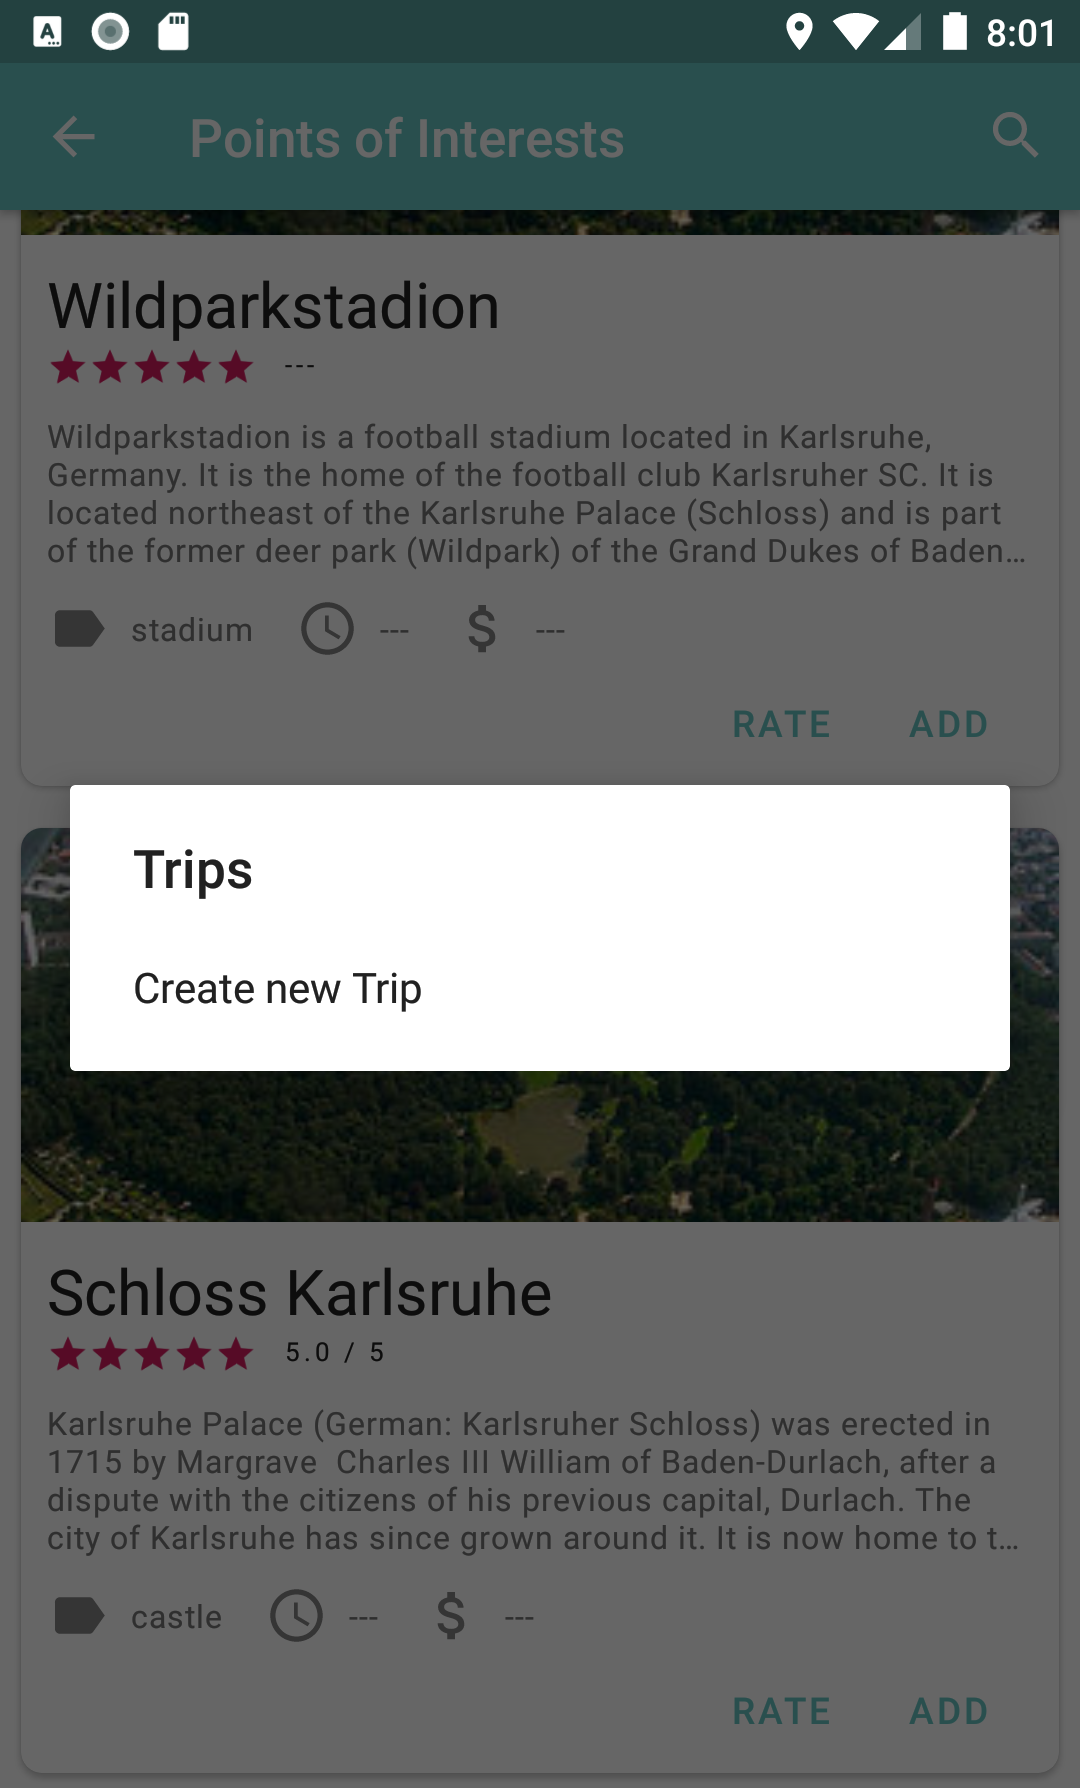
\includegraphics[width=0.32\textwidth]{images/travlyn-screenshot-stops-detail-selection-dialog.png}
		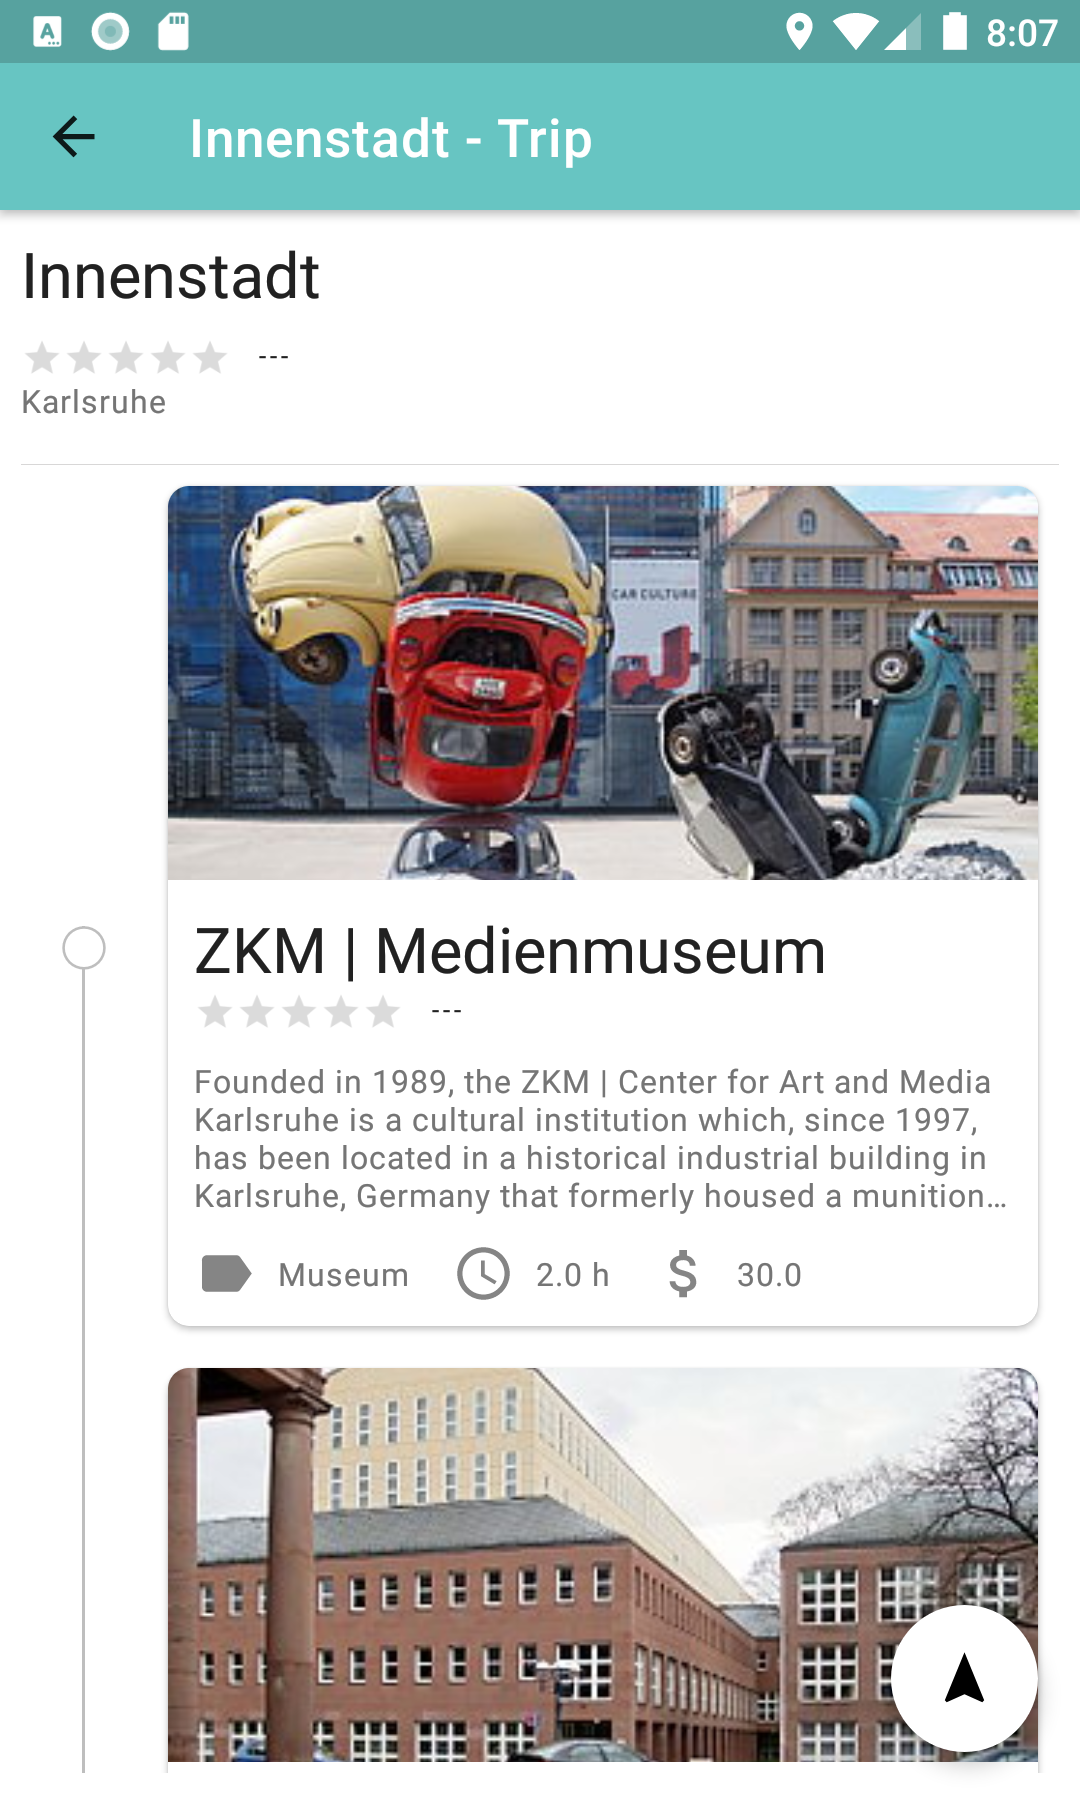
\includegraphics[width=0.32\textwidth]{images/travlyn-screenshot-trip-detail.png}
		\caption{Erstellung eines Trips anhand der bereitgestellten Stops}
		\label{fig:ui_trip_creation}
	\end{figure}

	\newpage
	
	\item \textbf{Trip Ausführung:} Am Urlaubsort angekommen können Trips ausgeführt werden. Es ist irrelevant, ob der auszuführende Trip ein eigener Trip ist oder ein öffentlicher Trip eines anderen Nutzers. Die Ausführung beinhaltet eine Navigation durch die Stadt, Informationen zu den einzelnen besuchten Sehenswürdigkeiten und die Möglichkeit die festgelegte Route zu verlassen und von der App trotzdem zum nächsten Stop geführt zu werden. Damit hat der Nutzer volle Flexibilität und eine sehr persönliche Reiseerfahrung.
	
	\begin{figure}[ht!]
		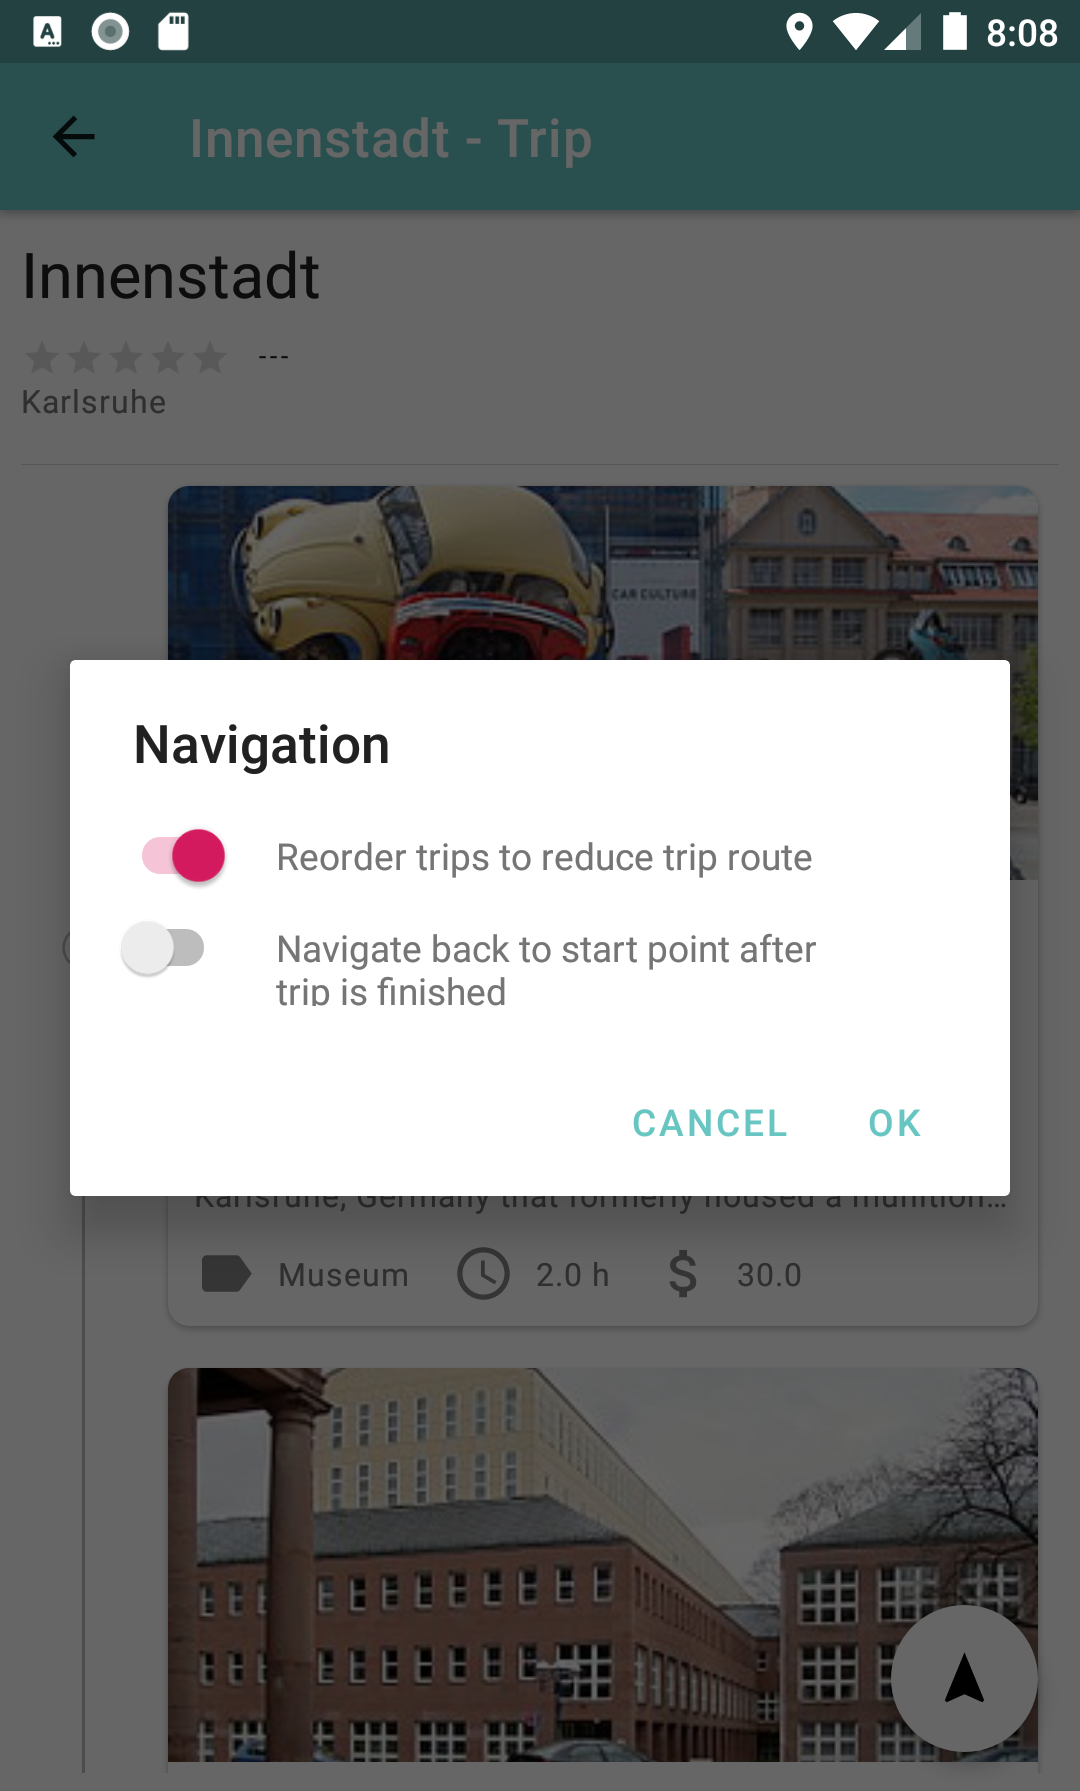
\includegraphics[width=0.32\textwidth]{images/travlyn-screenshot-start-navigation-dialog.png}
		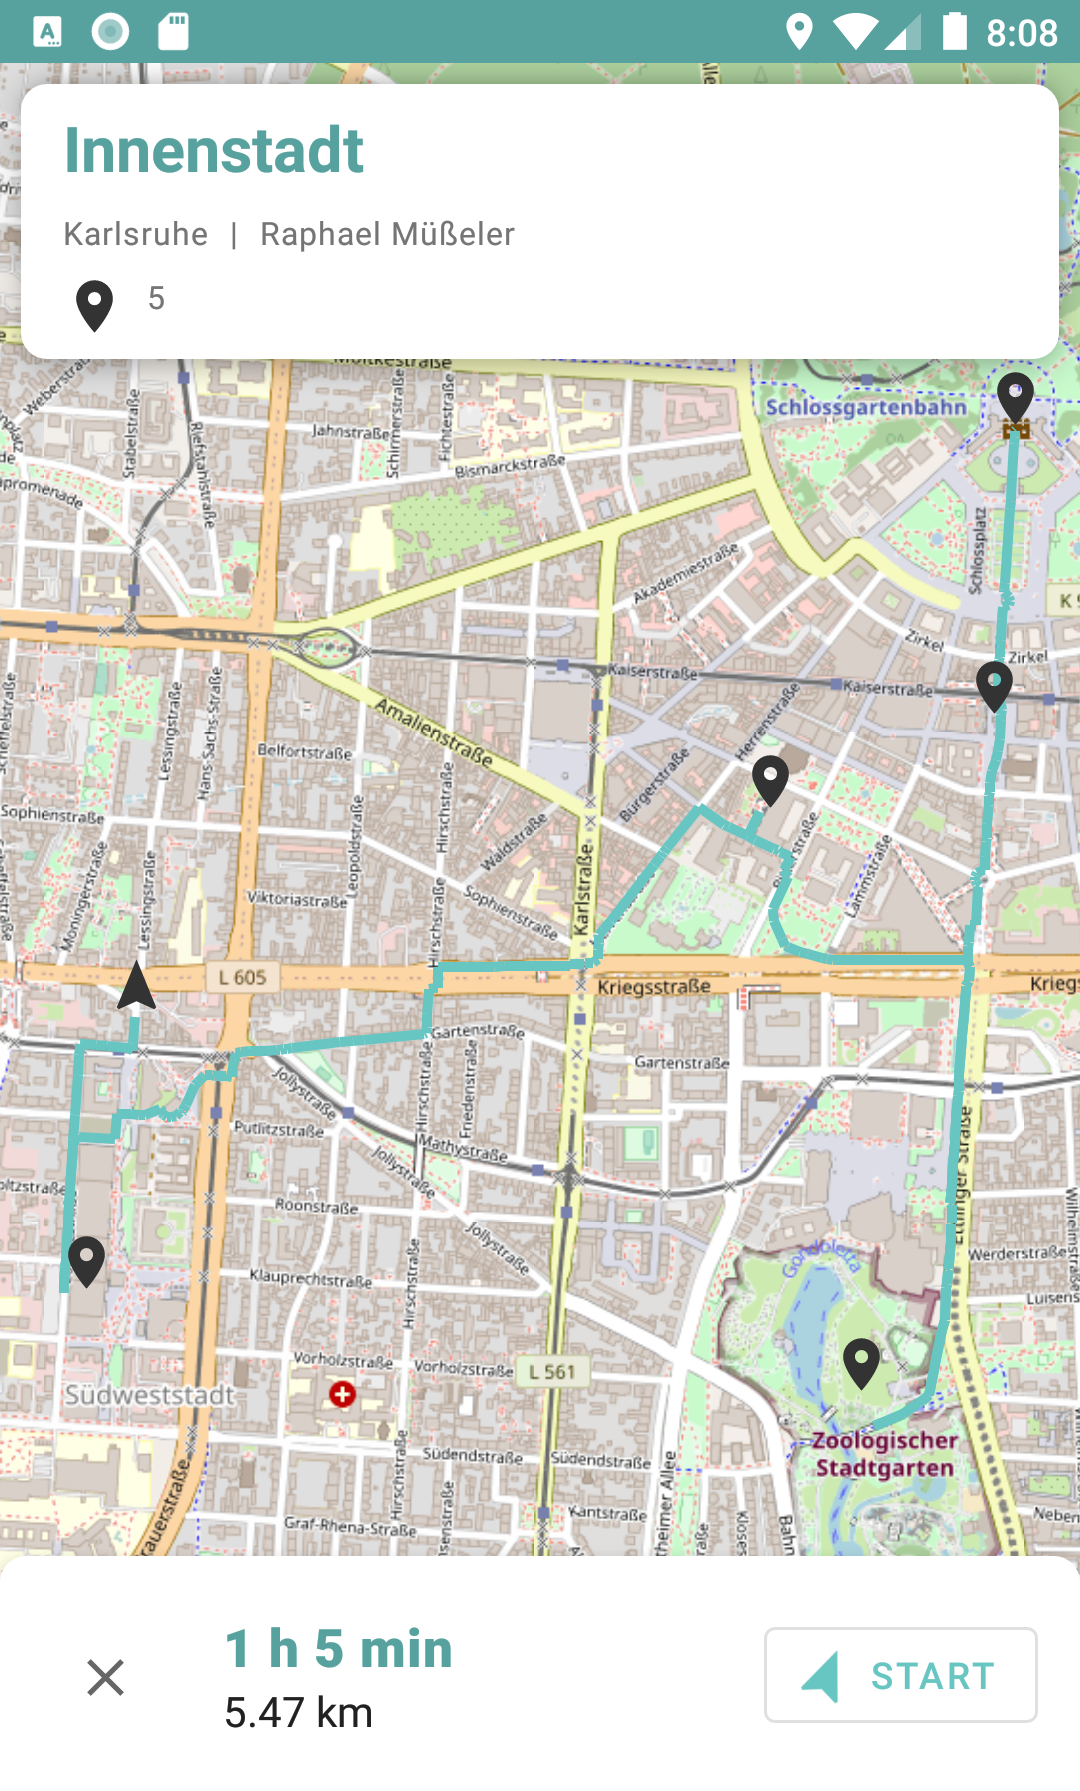
\includegraphics[width=0.32\textwidth]{images/travlyn-screenshot-navigation-overview.png}
		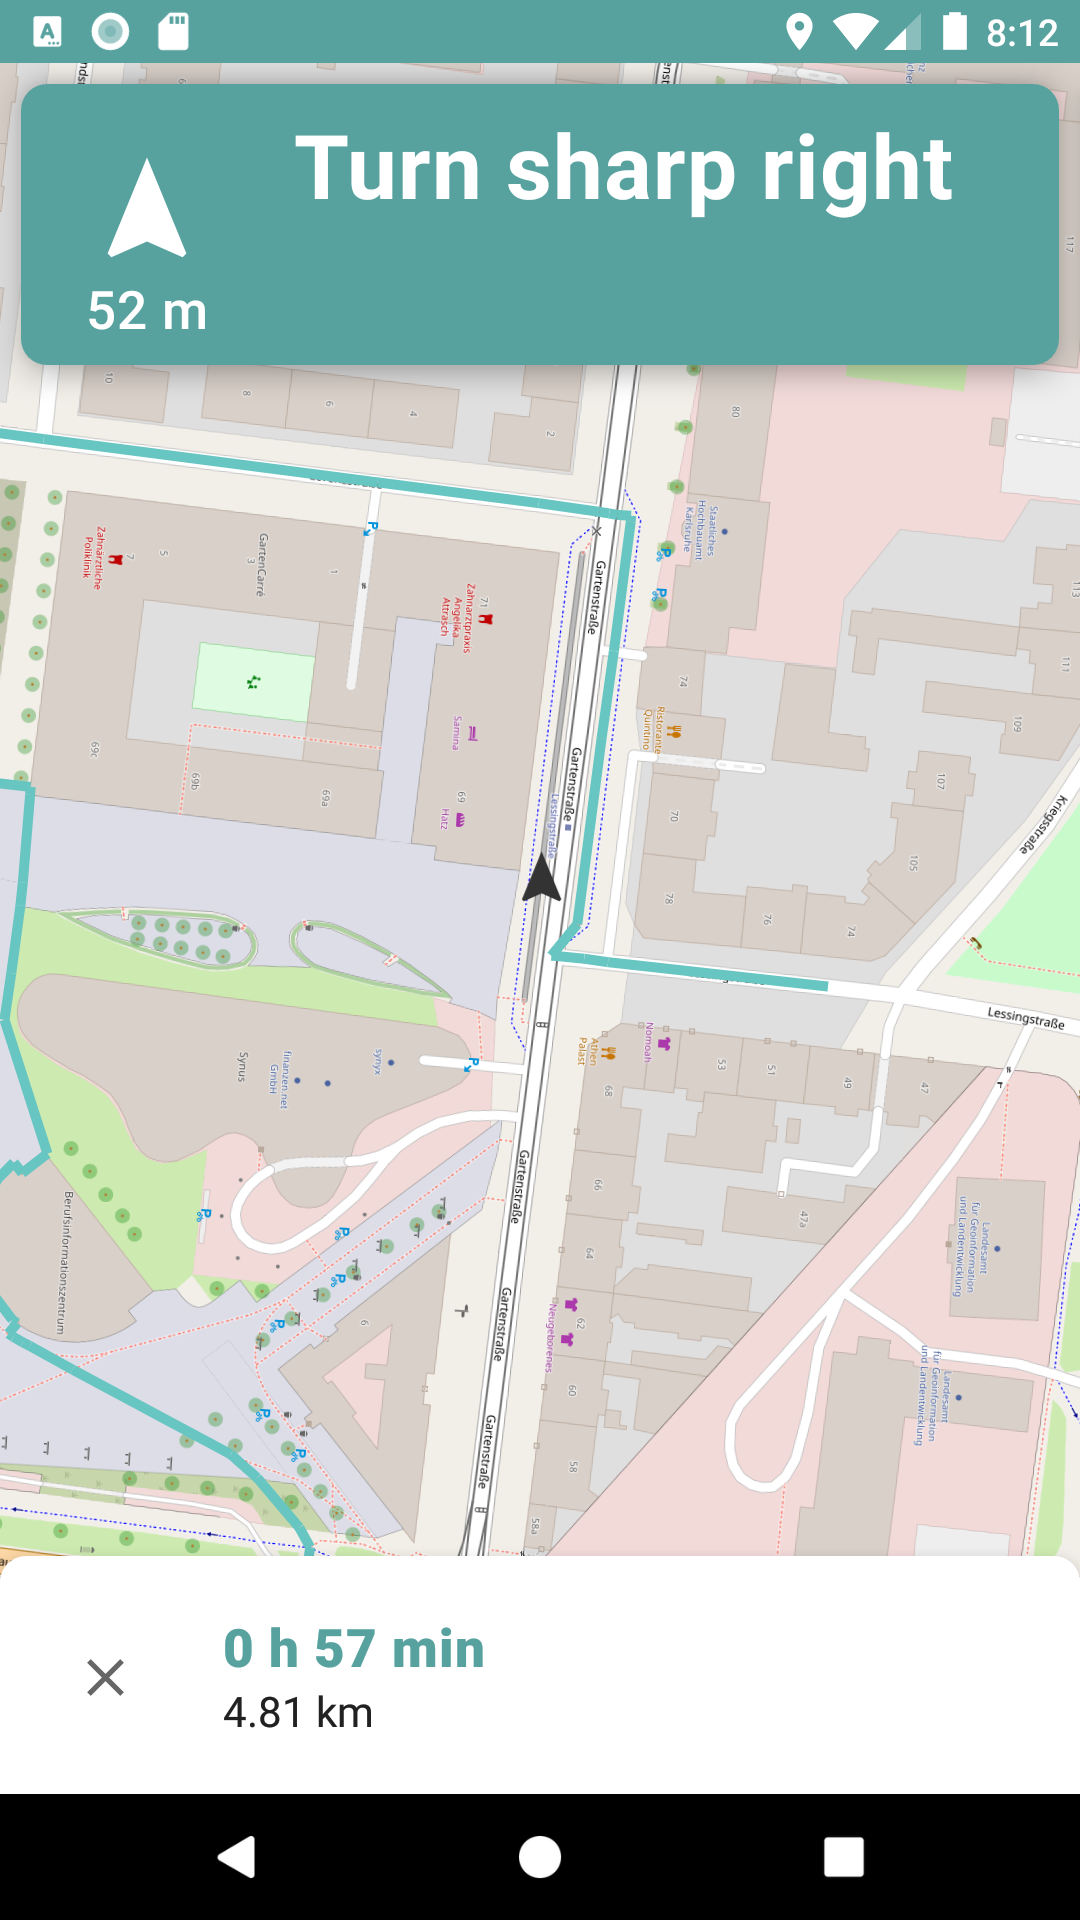
\includegraphics[width=0.32\textwidth]{images/travlyn-screenshot-navigation.png}
		\caption{Ausführung eines vorher erstellen Trips mit der \textit{Travlyn} App}
		\label{fig:ui_trip_execution}
	\end{figure}
    
\end{itemize}

Vergleicht man die beschriebenen Prozesse mit \autoref{fig:UCD} können alle Use Cases abgedeckt werden außer \textit{Share Trip}. Dieser Use Case war von Anfang an eher niedrig priorisiert und es hat sich im Verlauf der Arbeit herausgestellt, dass der Aufwand in keinem Verhältnis zum Ergebnis und somit wurde dieser Use Case nicht umgesetzt. Außerdem ist der Punkt \textit{Use API for custom purposes} und \textit{Get Trip Meta Data} nur als teilweise vollständig zu betrachten: Die erstelle API ist öffentlich zugänglich und kann mit einem API Schlüssel genutzt werden, allerdings gibt es keine automatische Generierung des Schlüssels. Diese Funktionalität ist für den Kern der \textit{Travlyn} App nicht von Bedeutung und wurde deshalb hinten angestellt.

\vspace{0.25cm}

Betrachtet man die API Use Cases als halb erfüllt, ergibt sich für die 10 übergeordneten Use Cases ein Erfüllungsgrad von 80\%, was als Erfolg gewertet werden kann, da ein Großteil der Nutzerprofile vollständig angeboten werden kann.

\section{Nicht-funktionale Anforderungen}
Neben den beschriebenen funktionalen Anforderungen wurden in \autoref{sec:anforderungen} auch nicht-funktionale Anforderungen gestellt, welche über die reine Funktionalität der App hinausgehen. Diese werden im Folgenden aufgegriffen und das entstandene Ergebnis gegen die Ziele validiert.

	\subsection{Benutzbarkeit}
	Als erste Anforderung wurde eine gute Benutzbarkeit und ein ansprechende Nutzungserfahrung gefordert, da die App auf mobilen Geräten mit kleinem Bildschirm und in Situationen genutzt wird bei denen die Konzentration eher auf der erlebten Reise und nicht auf der Bedienung der App liegen sollte und Schwierigkeiten mit der App die Erfahrung beeinträchtigen würden.
	
	\vspace{0.25cm}
	
	Zur Validierung dieses Ziels gibt es sehr viele Verschiedene Methoden, die unterschiedliche Vorteile und Herausforderungen bieten. Diese Methoden reichen von \textit{Lautem Denken}, über \textit{Konstruktive Interaktion} bis zu \textit{Usability Kiosks} \cite{Nielsen.20091993}. All diese Methoden liefern Usability-Daten die zum einen durch die Auswertung der Äußerungen der Nutzer und zum anderen durch verschiedene Metriken wie z.B. die benötigte Zeit für eine Aktion, die Anzahl der begangenen Fehler oder die Anzahl der ungenutzt gebliebenen Features interpretiert werden. Es gibt feste Methoden zum planen und durchführen dieser Tests.
	
	\vspace{0.25cm}
	
	Auf Grund der aktuellen Situation, die durch das COVID-19 Virus geprägt ist und dem engen Zeitplan für diese Arbeit, können leider viele der von \cite{Nielsen.20091993} vorgestellten Methoden nicht ausgeführt werden, da ein direkter Kontakt zu den Testnutzer erforderlich wäre. Somit ist es notwendig ein kontaktloses und vom Umfang angemessenes Verfahren zu finden, welches einen wissenschaftlich begründeten Überblick über die erreichte Usability bietet.
	
	Schlussendlich viel die Entscheidung auf die \ac{SUS} \cite{Brooke.1996}. Diese Skala wurde von John Brooke entwickelt und konzentriert sich auf einen schnellen und kostengüstigen Test der Usability. Ursprünglich entstand diese Umfrage im Bereich der Industrie, in der oft schnelle und grundlegende Usability-Bewertungen benötigt werden, ohne dass viele Testpersonen über Stunden befragt werden müssen oder komplizierte Auswertungen durchgeführt werden müssen. Trotz den beschriebenen Abstrichen hat sich diese Methode in der Industrie durchgesetzt und ist weit etabliert \cite{MatthiasRauer.11.April}. Dieses Verfahren stellt einen Usability-Wert durch eine Umfrage fest, die zehn Fragen beinhaltet. Diese werden von Testpersonen beantwortet, die vorher die Möglichkeit hatten das betreffende System zu testen, aber bevor Diskussionen mit anderen Testpersonen stattfinden. Die Antworten sollen intuitiv und ohne Nachdenken gegeben werden \cite{Brooke.1996}. Die Fragen bestehen aus grundlegenden Bewertungsfragen in denen Aussagen wie z.B:
	
	\begin{itemize}
		\item \enquote{Ich kann mir sehr gut vorstellen, das System regelmäßig zu nutzen.}
		\item \enquote{Ich empfinde das System als einfach zu nutzen.}
	\end{itemize}

bewertet werden sollen (restliche Fragen siehe \cite{Brooke.1996}). Hierfür steht eine Likert-Skala \cite{Joshi.2015} zur Verfügung, die fünf bis sieben Auswahlmöglichkeiten von \enquote{Starke Zustimmung} bis \enquote{Überhaupt keine Zustimmung} enthält.

\vspace{0.25cm}

Nach der Durchführung der Umfrage werden alle Ergebnisse anhand eines fest vorgegebenem Verfahren verrechnet: Für einen Teil der Fragen gilt die abgegebene Punktzahl der Likert-Skala minus eins und für den anderen Teil fünf minus den abgegeben Punktwert. Nach der Summation aller Werte und dem Multiplizieren mit der Konstante 2.5 ergibt sich ein Ergebniswert zwischen 0 und 100, welcher die Usability widerspiegelt und vergleichbar macht.

\vspace{0.25cm}

Da die Durchführung der Befragung sehr einfach alleine online und ohne weitere Einflussnahme der Tester/Entwickler durchgeführt werden kann und trotzdem ein wissenschaftlich anerkanntes Ergebnis liefert wurde für \textit{Travlyn} ein Test mit der \acs{SUS} durchgeführt. Im Folgenden wird die konkrete Durchführung dieses Verfahrens aufgezeigt.    
	
		\subsubsection{Aufbau}
		Zur Vorbereitung des Experiments wurde ein Server mit dem \textit{Travlyn}-Backend aufgesetzt und die App als \acs{APK}-Datei erstellt. Durch den Jenkins-Buildserver war diese automatische Erstellung sehr einfach und schnell. Des Weiteren wurden geeignete Testpersonen ausgesucht: Da die Zielgruppe der Applikation jeden umfasst der gerne reist, kamen viele Personen aus dem Umfeld des Entwicklungsteams infrage. Ausgewählt wurde schließlich eine Gruppe von 15 Testpersonen, die einen Durchschnitt über das Alter bilden (von 14 bis Ende 50) und alle Nutzergruppen von praktisch keiner Technikerfahrung bis ausgiebiger täglicher Technikerfahrung abdecken. Für die Online Befragung wurde das zu Google gehörende Tool \textit{Google Forms} verwendet \cite{Google.2020}.
		
		\subsubsection{Ablauf}
		Nach der Auswahl und Erstellung aller oben beschrieben Artefakte wurde eine Mail mit der Applikationsdatei und dem Link zur Umfrage an alle Testpersonen verschickt. Alle Testpersonen sollen die Applikation selbständig installieren und nach Belieben ausprobieren. Im direkten Anschluss soll der bereitgestellte Link genutzt werden, um die Onlineumfrage auszufüllen. Bei technischen Problemen standen die Entwickler über digitale Kanäle zur Hilfe bereit.
		Durch die Nutzung des Google Tools läuft die Zusammenstellung der Ergebnisse automatisch ab und kann gesammelt abgerufen werden.  
		\subsubsection{Ergebnis}
		Die abgerufenen Ergebnisse wurden wie oben beschrieben verrechnet, pro Frage wird die durchschnittliche Antwort errechnet und entsprechen der zwei Rechenregeln ein endgültiger Wert bestimmt (Fragen 1, 3, 5, 7 und 9: Antwort minus eins; Fragen 2, 4, 6, 8 und 10: fünf minus den Antwortwert). Damit ergeben sich folgende Werte:
		
		\begin{itemize}
			\item \textbf{Frage 1:} Durchschnitt: 4.666, damit endgültiger Wert: 3.666
			\item \textbf{Frage 2:} Durchschnitt: 1.467, damit endgültiger Wert: 3.533
			\item \textbf{Frage 3:} Durchschnitt: 4.467, damit endgültiger Wert: 3.467
			\item \textbf{Frage 4:} Durchschnitt: 1.267, damit endgültiger Wert: 3.733
			\item \textbf{Frage 5:} Durchschnitt: 4.733, damit endgültiger Wert: 3.733
			\item \textbf{Frage 6:} Durchschnitt: 1.333, damit endgültiger Wert: 3.667
			\item \textbf{Frage 7:} Durchschnitt: 4.667, damit endgültiger Wert: 3.667
			\item \textbf{Frage 8:} Durchschnitt: 1.333, damit endgültiger Wert: 3.667
			\item \textbf{Frage 9:} Durchschnitt: 4.4, damit endgültiger Wert: 3.4
			\item \textbf{Frage 10:} Durchschnitt: 1.067, damit endgültiger Wert: 3.933
		\end{itemize}
	
	Zur Berechnung des Skalawerts zwischen 0 und 100 werden alle endgültigen Werte aufsummiert und mit 2,5 multipliziert:
	
	\begin{itemize}
		\item Summe: 37.8725, damit Usabilityscore: $36.466*2.5=91.165$
	\end{itemize}

	Der vorliegende Usabilityscore von 91.165 liegt im obersten Zehntel der Skala. Dies kann als Zeichen für eine sehr gute Benutzbarkeit gesehen werden. Diese Bewertung zeigt, dass die Testnutzer die Applikation als leicht und intuitiv benutzbar empfunden haben, was eine zwingende Eigenschaft für gute Software-Produkte ist. Die größte Streuung der Antworten ist bei der Frage acht aufgefallen: \enquote{Ich fühle mich sicher, wenn ich die App benutze.}. Um diesem einen Nachteil entgegenzuwirken sollte in Zukunft auf eine adäquate Fehlerbehandlung und vor allem einer guten Nutzerunterstützung im Fehlerfall geachtet werden.
	
	\vspace{0.25cm}
	
	Trotz der oben genannten Verbesserungsmöglichkeit erfüllt der sehr hohe Usability-Score die Anforderungen an eine gute Benutzbarkeit der \textit{Travlyn} Applikation und somit gilt dieses nicht-funktionale Ziel als erfüllt. 
	
	\subsubsection{Weitere Hinweise}
	Wie in \cite{Nielsen.20091993} beschrieben gibt es im Usability-Testing einige Fallstricke und viele Methoden haben Probleme mit Zuverlässlichkeit und Validität. Somit ist nicht zwingend sichergestellt, dass diese Usability-Experimente bei wiederholter Ausführung das gleiche Ergebnis ergibt und ob das Ergebnis des Experiments wirklich die zu testende Eigenschaft widerspiegelt. Somit ist das obenstehende Ergebnis als Orientierung zu erachten und müsste durch weitere Tests, welche wir unter den aktuellen Umständen leider nicht durchführen können, validiert werden.
	
	\subsection{Sicherheit}
	Um die Sicherheit des Codes zu überprüfen wurden diverse Methoden eingesetzt, welche in \autoref{sec:QM} beschrieben wurden. Die erste ebene ist die Testebene: Es wurde Wert auf Tests gelegt, welche möglichst viele Szenarios und vor allem Fehlerfälle abdeckt, damit wird sicher gestellt, dass die einzelnen Einheiten sich im Falle einer unerwarteten Situation richtig verhalten und somit nicht angreifbar sind. Beispielsweise wird auf den entsprechenden Trip Endpoints getestet, dass ein Nutzer nur auf private Trips zugreifen kann, wenn er eingeloggt ist und einen Trip abruft, der seinem Account zugeordnet ist.
	
	\vspace{0.25cm}
	
	Neben den Tests gibt es mit SonarQube eine weitere technische Kontrollinstanz. Dieses Tool analysiert, wie in \autoref{qm.sonarqube} beschreiben, statisch den Code um nach Fehlern und vor allem Verwundbarkeiten und Bugs zu suchen. Durch diese Analyse sind während der Implementation immer wieder Konstrukte aufgefallen, welche eine Angriffsmöglichkeit dargestellt hätten. Durch die Detektion von SonarQube konnten diese Fehler allerdings behoben werden, sodass \textit{Travlyn} nun den Top zehn Sicherheitsstandards der OWASP Foundation \cite{OWASPFoundation.20200503T01:28:27.000Z} genügt. \autoref{fig:sonarqube_result} zeigt diese Top zehn Liste und dass keine entsprechende Stelle im Code gefunden wurde.
	
	\begin{figure}[ht!]
		\centering
		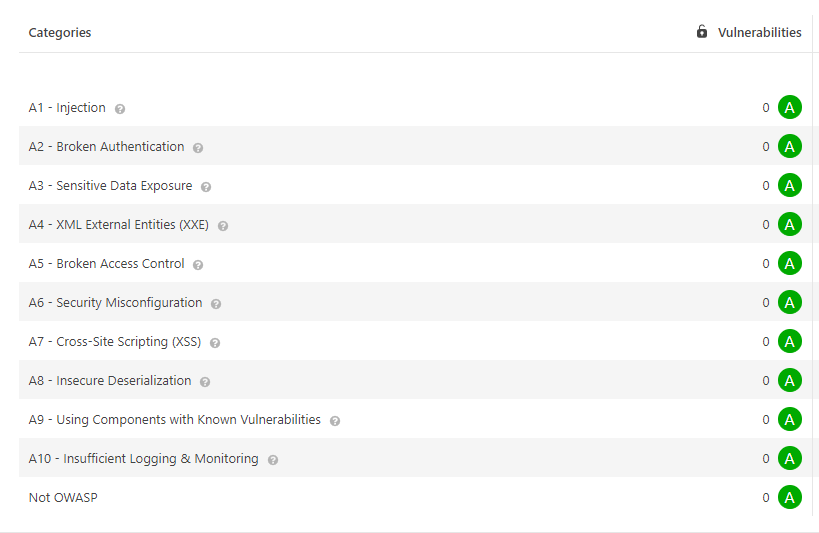
\includegraphics[width=1\textwidth]{images/Verwundbarkeiten_SonarQube.png}
		\caption{Erkannte Verwundbarkeiten durch SonarQube}
		\label{fig:sonarqube_result}
	\end{figure}

	Neben den technischen Möglichkeiten wurde der erstellte Code während der Entwicklung regelmäßig durch gemeinsame Reviews durch die Entwickler validiert. Wie in \autoref{sec:QM} beschrieben wurde jeder Pull Request vor dem Einfügen in den Master-Branch reviewed und bei entsprechenden Fehlern und Unklarheiten solange geändert, bis alle Zweifel ausgeräumt waren. Somit genügt der Code dem \enquote{Vier-Augen-Prinzip} und Fehler welche die technischen Hilfsmittel nicht aufdecken konnten wurden in diesem Prozess gefunden.
	
	\vspace{0.25cm}
	
	Somit gibt es eine ausgiebige Kontrolle des Code, welcher sicherstellt, dass keine Verwundbarkeiten vorliegen. Das Ziel eine gute Sicherheit für \textit{Travlyn} zu garantieren ist damit erreicht, allerdings ist Sicherheit kein dauerhafter Zustand und muss laufend neu beurteilt und erarbeitet werden.
	
	\subsection{Wartbarkeit}
	Neben der Sicherheit ist die Wartbarkeit stark von der Code Qualität abhängig. Die Methoden zur Sicherstellung der Wartbarkeit überschneiden sich teilweise mit denen die Sicherheit sicherstellen und sind in \autoref{sec:QM} dargestellt. Für \textit{Travlyn} spielt SonarQube auch hier eine große Rolle, da es ein Code Quality Gate zur Verfügung stellt, welches von Code erfüllt werden sollte, damit eine hohe Code Qualität und Wartbarkeit gegeben ist.
	
	\begin{figure}[ht!]
		\centering
		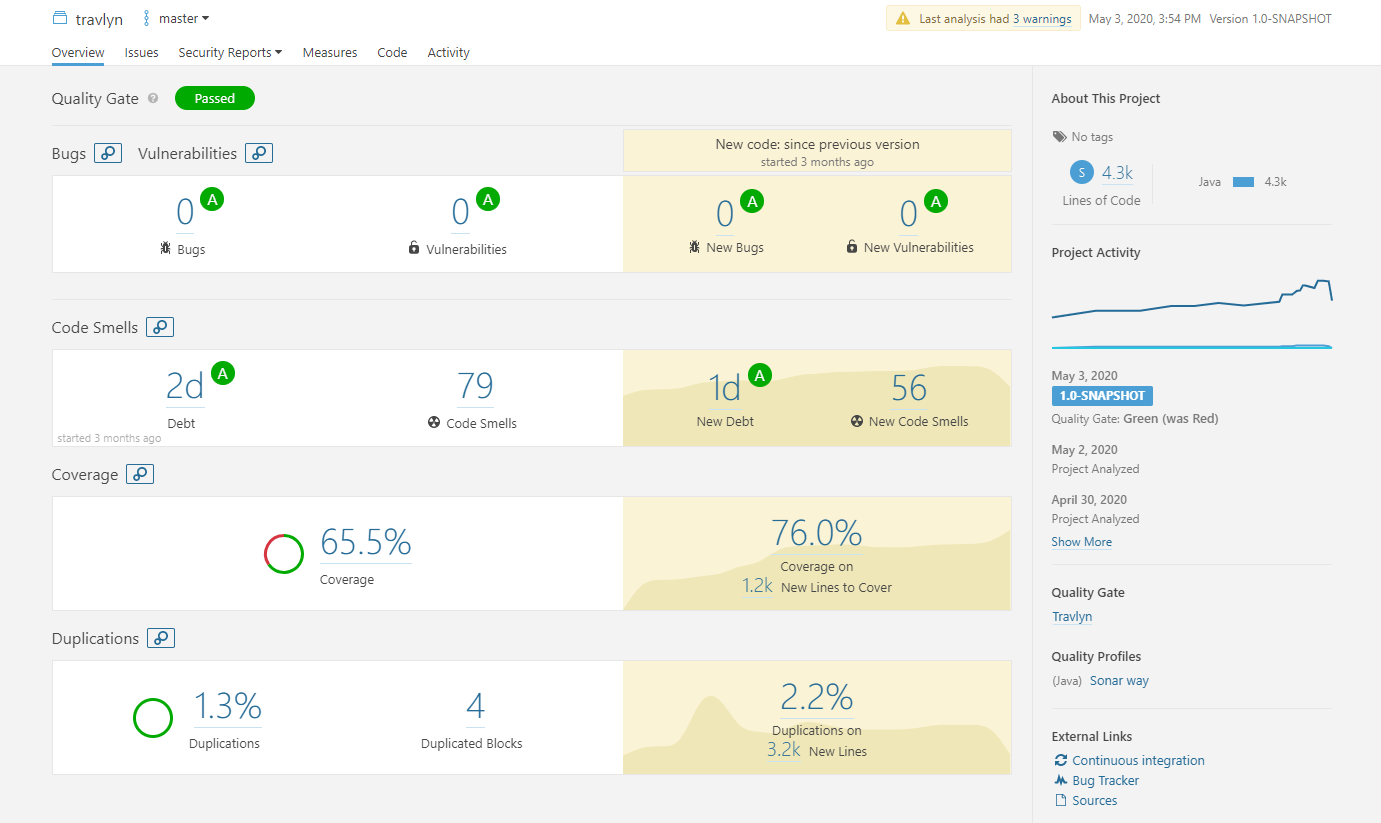
\includegraphics[width=1\textwidth]{images/sonar_passed_QG.png}
		\caption{Evaluation des Codes im Hinblick auf das Quality Gate in SonarQube}
		\label{fig:soarqube_QG}
	\end{figure}

	\autoref{fig:soarqube_QG} zeigt die Auswertung des \textit{Travlyn} Codes. Es ist zu erkennen, dass der Code dem Quality Gate genügt. Damit sind die folgenden Qualitätsmerkmale für Quellcode sichergestellt:
	
	\begin{itemize}
		\item Der Code beinhaltet keine Bugs oder Verwundbarkeiten (siehe oben).
		\item Der Code hat eine angemessene Komplexität und nur wenige stellen mit schlecht strukturiertem Code (siehe \textit{Code Smells}).
		\item Die Testabdeckung ist hoch (hier über 65\%) und kann eine korrekte Funktionsweise des Codes sicherstellen.
		\item Es gibt kaum duplizierte Code stellen, welche die Pflege erschweren würden. 
	\end{itemize} 
	
	\newpage
	
	Neben der technischen Prüfung des Codes ist auch hier die Nutzung der Code Reviews hervorzuheben. Durch das oben beschriebene Verfahren konnte vermieden werden, dass nur der Ersteller eines spezifischen Code Blocks den Aufbau und Ablauf kennt, da mindestens ein zweiter Entwickler sehr tief in den Code eingestiegen ist und eine gute Lesbarkeit für Dritte sichergestellt hat. Damit können mehrere Entwickler die Funktionalität erweitern und Fehler beheben, was für eine gute Wartbarkeit sorgt.
	
	\subsubsection{Logger}
	Zum finden von Fehlern, welche im laufenden Betrieb auftreten wurde auf ein ausgiebiges Logging gesetzt, welches alle Aktionen auf dem Server registriert und persistiert. Die einsehbaren Log-Files können zur Fehleranalyse und der Ursachenfindung genutzt werden. Damit ist die akute Fehlerbehandlung sehr vereinfacht. 
	
	\vspace{0.25cm}
	
	Insgesamt sind die in \autoref{sec:anforderungen} beschriebenen Ziele zur Wartbarkeit damit gut erfüllt und werden ständig neu überprüft. Wartbarkeit ist ebenso wie Sicherheit kein dauerhafter Zustand und es gilt bei weiteren Entwicklungen die Wartbarkeit weiterhin aktiv und durch regelmäßiges anpassen des Codes sicherzustellen.
	
	
	
	\subsection{Datenquellen}
	Aufgrund der begrenzten Ressourcen war die Auswahl der Datenquellen für dieses Projekt besonders kritisch: Es sollten keine Kosten anfallen und schwierige Lizenzfragen vermieden werden, um die Möglichkeit einer späteren Veröffentlichung der Applikation zu schaffen. Wie bereits in \autoref{sec:datengrundlage} beschrieben wurden die Quellen für \acs{POI}s und weiteren Informationen wie Kartendaten nach den gestellten Zielen ausgewählt. Nach Abschluss des Projekts ist festzuhalten, dass der Großteil der funktionalen Anforderungen mit diesen teilweise begrenzten Informationsquellen umgesetzt werden konnte (siehe \autoref{sec:funktional_evaluation}).
	
	\vspace{0.25cm}
	
	Neben der Auswahl der Datenquellen wurde auch die Auswahl der verwendeten Bibliotheken und Frameworks aufgrund dieser Ziele getroffen. So wurde sich z.B. explizit gegen ein UI Framework zur Visualisierung der Routenführung entschieden, welches nur für einen sehr begrenzten Nutzerkreis im Monat kostenlos gewesen wäre und es wurde eine eigene Implementation erstellt, welche die Crowd Sourced Daten von \acs{ORS} verwendet und visualisiert. Falls es geeignete Open Source Bibliotheken für das betreffende Thema gab, wurden diese eingesetzt, um den Aufwand einer eigenen Implementation zu sparen.
	
	\vspace{0.25cm}
	
	Aufgrund der Durchsetzung der oben genannten Maßnahmen könnte die App im aktuellen Zustand von rechtlicher Perspektive sicher veröffentlicht werden und auch für kommerzielle Zwecke genutzt werden, ohne das Risiko von Ansprüchen der Datenanbieter einzugehen. Trotz dieser Einschränkungen sind ansprechende Nutzungsmöglichkeiten entstanden, denen es nicht an Daten oder Funktionalität mangelt. Damit sind die Ziele für Datenquellen in diesem Projekt vollständig erfüllt.
	
	\subsection{Zuverlässigkeit}
	
	Die zu Beginn der Arbeit geforderte Zuverlässigkeit der \textit{Travlyn} Applikation liegt nur zum Teil in den Händen der Entwickler. Die Infrastruktur auf der sowohl das Backend, als auch das Frontend laufen sind nicht unter direkter Kontrolle des Entwicklungsteams, sondern in Händen der Serververmietung bzw. der tatsächlichen Nutzer. Somit muss sich grundsätzlich auf diese Gruppen verlassen werden.
	
	\vspace{0.25cm}
	
	Um diese Gruppen, insbesondere die Nutzer, zu unterstützen wurde bei der Entwicklung des Codes auf eine adäquate Fehlerbehandlung, hohe Kompatibilität und einen angemessenen Ressourcenverbrauch geachtet. Damit soll zum einen verhindert werden, dass die Infrastruktur durch \textit{Travlyn} überlastet wird und dadurch weniger Zuverlässig wird. Zum anderen sollen sowohl der Server als auch der Client nach einem möglichen Fehler einfach wieder startbar sein, ohne einen großen administrativen Aufwand zu verursachen und beim Nutzer ggf. die Hilfe einer technischen Supportperson erfordern. Damit ist sichergestellt, dass im unwahrscheinlichen Fehlerfall die Ausfallzeit sehr begrenzt ist und schnell behoben werden kann.  
	
	\section{Übergeordnete Visionen}
	
	Neben den granularen Anforderungen soll abschließend auf die übergeordnete Vision eingegangen werden. Diese wurde am Anfang von \autoref{sec:anforderungen} beschrieben:
	
	\vspace{0.25cm}
	
	\enquote{Durch \textit{Travlyn} sollen Nutzer in der Lage sein, ihre Städtereisen ohne das Mitführen von papierbasierten Reiseführern oder die Nutzung von multiplen mobilen Diensten zu bewältigen, ohne dabei einen Informationsverlust oder eine Beeinträchtigung des Reisespaßes hinnehmen zu müssen.}
	
	\vspace{0.25cm}   
	
	Rückblickend treten bei der Realisierung einige Probleme auf, welche während der Entwicklung aufgedeckt wurden. So gibt es zwar eine große Anzahl von verfügbaren Datenquellen, welche unterschiedlichen Ansprüchen genügen (z.B. frei verfügbar für kommerzielle Nutzung). Allerdings sind diese Quellen meist entweder lokal oder thematisch begrenzt, was zu der Nutzung von sehr vielen Datenquellen für einen kompletten digitalen Reiseführer führen würde. Zum anderen ist die Verbindung der Informationen von verschiedenen Quellen u.U. schwierig (siehe \autoref{sec:mapping}).
	Ein zweites gravierendes Problem ist die fehlende Digitalisierung anderer Lebensbereiche. Da viele Informationen, die zum Reisen relevant sind, nicht digital verfügbar sind (z.B. Öffnungszeiten, Preise und \enquote{Geheimtipps} von Ortsansässigen) können sie auch nicht ohne großen redaktionellen Aufwand in einen digitalen Reiseführer integriert werden. Vor allem der Anspruch eines Reiseführers der weltweit nutzbar ist somit noch kritischer zu sehen, da es viele Länder gibt in denen bis jetzt praktisch keine Digitalisierung stattgefunden hat.
	
	\vspace{0.25cm}
	
	Trotz dieser aufgetretenen Probleme konnte im Zuge dieser Arbeit einen Applikation entwickelt werden, welche zumindest den Weg zu einem digitalerem Reisen aufzeigt, indem mehrere Informationsquellen kombiniert werden, über moderne Infrastruktur verfügbar gemacht werden und über mobile Darstellungsmöglichkeiten von jedem Nutzer mit Smartphone abgerufen werden können.
	
	Die App bietet eine Informationsfülle für viele Städte und Sehenswürdigkeiten (mit Ausnahme derer, die unter die oben genannten Probleme fallen) und bietet Fähigkeiten, die kein papierbasierter Reiseführer je bieten kann, wie z.B. die interaktive Navigation durch eine Stadt abhängig von der eigenen Position oder das Zusammenstellen und Speichern von personalisierten Rundtrips. Somit wird auch eine Reise mit der \textit{Travlyn} App einen Reiz und Reisespaß bieten.
	
	\vspace{0.25cm}
	
	Insgesamt konnte mit dieser Arbeit ein guter Grundstein für eine ausführliche Erfüllung der zugrunde liegenden Vision geschaffen werden, auch wenn sicherlich nicht alle Probleme durch die \textit{Travlyn} Applikation voll umfassend gelöst werden konnten. Somit ist eine Eindeutige Empfehlung zur Nutzung der Applikation zu formulieren,  mit dem eindeutigen Hinweis, dass die Nutzung eines papierbasierten Reiseführers bis jetzt nicht komplett ersetzt werden kann und weiterhin seine Berechtigung behält.
\chapter{Fazit}

	(Raphael)

	\textit{Travlyn} ist ein intelligenter Reiseführer, der es ermöglicht, mithilfe externer \acs{API}s wie OpenRoute Service und DBpedia Informationen zusammenzutragen und dem Nutzer zu Verfügung stellt. Der Nutzer kann dann aus diesen Informationen Trips generieren, welche dann den Nutzer durch die Stadt navigieren und zusätzliche Informationen wie eine ausführliche Beschreibung der Sehenswürdigkeiten anzeigen. 
	
	\textit{Travlyn} wurde im Rahmen einer Studienarbeit erfolgreich umgesetzt. Die zuvor definierten funktionalen und nicht-funktionalen Anforderungen wurden -- bis auf kleinere Ausnahmen -- vollständig umgesetzt. Durch eine Usability-Evaluation wurde außerdem gezeigt, dass das Zusammenspiel zwischen User Interface und Funktionalität sehr gut umgesetzt wurde. Abschließend lässt sich sagen, dass \textit{Travlyn} ein erfolgreiches Projekt mit vielen lehrreichen Elementen aus dem Bereich der Software-Engineering aber auch der Algorithmik war. 
	
	Das Projekt \textit{Travlyn} brachte alle an diesem Projekt beteiligten Entwickler in ihrer beruflichen Laufbahn durch den Erwerb von neuem Wissen sowie der praxisbezogenen Anwendung weiter und könnte außerdem die Basis für weitergehende Projekte oder Erweiterungen sein. 


% ---- Literaturverzeichnis
\cleardoublepage
\renewcommand*{\chapterpagestyle}{plain}
\pagestyle{plain}
\pagenumbering{Roman}                   % Römische Seitenzahlen
\setcounter{page}{\numexpr\value{savepage}+1}
\printbibliography[title=Literaturverzeichnis]

% ---- Anhang
\appendix
%\clearpage
%\pagenumbering{Roman}  % römische Seitenzahlen für Anhang

\newpage
\end{document}
